\documentclass[fleqn,parskip=half]{scrbook} % <= Druckversion: "scrbook" / Bildschirmversion: "scrreprt"
\usepackage[ngerman,biber]{hpi-praeambel} % <= Sprache der Arbeit ("ngerman"/"english"), Biblatex-Backend ("bibtex"/"biber")

% ABOUT
% Eingabe anpassen
% Quelle Literaturverzeichnis oder URL in Fussnote 
%\newcommand{\quelle}{\quelle}{Jan Schaffranek franneck94~\footnote{\url{https://github.com/franneck94}}}
%\newcommand{\quelle}{MathePeter siehe~\textcite{peter:2021:mathe}}% Literaturverzeichnis
\newcommand{\fach}{IT}
\newcommand{\titel}{Microsoft Windows Server für Einsteiger}
\newcommand{\untertitel}{}
\newcommand{\typ}{Notizen}% \LaTeX 
\newcommand{\autor}{Jan Unger}
\newcommand{\datum}{\today}
\newcommand{\datumHand}{18.12.2021}% ##.##.####
\newcommand{\website}{https://bw-ju.de}
\newcommand{\websiteKurz}{bw-ju.de} 

% DOCUMENT
\bibliography{content/literatur}
\bibliography{content/literatur-kfz}
\bibliography{content/literatur-sport}


\begin{document}
	
	% (Haupt-)Titelseite, Abstract, ggf. Danksagung & Inhaltsverzeichnis
	\pagenumbering{roman}
	\begin{titlepage}

	% background picture
	\begin{tikzpicture}[overlay, remember picture]
	\node[anchor=north east, 
		xshift=+0.2cm, 
		yshift=+0.2cm] 
		at (current page.north east)
		{
\includegraphics[width = 1.54\linewidth]{images/titelbild}};%titelbild 
	\end{tikzpicture}

	\centering	
	\vspace*{12\baselineskip}


	% oder background picture
	%
\includegraphics[width=\textwidth]{images/titelbild}
	%\vspace*{4\baselineskip}

	{\usekomafont{subject}\typ}\par
	\vspace*{\baselineskip}
	{\usekomafont{title}\titel}\par
	\vspace*{\baselineskip}
	{\usekomafont{subtitle}\fach}\par
	\vspace*{\baselineskip}
	{\smallskip\usekomafont{author}\autor}\par
	{\usekomafont{date}\datum}\par
	
	\vfill

	\setcounter{page}{1}

\end{titlepage}



	\ifisbook\cleardoubleemptypage\fi% deutsche Zusammenfassung
\null\vfil
\begin{otherlanguage}{ngerman}
\begin{center}\textsf{\textbf{\abstractname}}\end{center}

    %\noindent

    \begin{quote}
        \textcolor{purple}{>>Die Mathematik ist die Sprache der Natur, 
        ihre Buchstaben sind Dreiecke, Kreise und andere Figuren.<<}\\ 
        \raggedleft \small{-- Galileo Galilei}% 10pt
        
        \raggedright
        \textbf{Dozent:} Mustermann

        \textbf{Bücher:}

        \begin{itemize}
            \item Motormanagement Sensoren, \textcite{schneehage:2021:motormanagement}.
        \end{itemize}


    \end{quote}

\end{otherlanguage}
\vfil\null




	\tableofcontents
	\cleardoublepage

	% Textteil
	\pagenumbering{arabic}

	%\chapter{Checkliste}
	% Check anpassen
	%\begin{itemize}[label=\checkmark] \itemsep -2pt
	%	\item Check 
	%\end{itemize}
	
	% Textteil anpassen

	%Randnotiz
	%\todo{Make a cake \ldots}

	%Fußnote~\footnote{Text der Fußnote.} 

	%\textbf{Quelle:} \quelle

	%Meine Website~\footnote{\url{\website}}

	%%%%%%%%%%%%%%%%%%%%%%%%%%%%%%%%%%%%%%%%%%%%%%%%%%%%%%%
	
	%%%%%%%%%%%%%%%%%%%%%%%%%%%%%%%%%%%%%%%%%%%%%%%%%%

% Latex Kapitel erstellen. 
% 		Kopiere 'texPandoc/*.tex' nach 'content/tex' 
% 		'content/tex' **Handarbeit... für opt. Ergebnisse!** 
% 		Kopiere 'archiv/inhalt.tex' nach 'content/' 
% 		make -- Latex-PDF erstellen 
% ju 05-Feb-2022 inhalt.tex

%%%%%%%%%%%%%%%%%%%%%%%%%%%%%%%%%%%%%%%%%%%%%%%%%%

% content/

%\chapter{01_beamer}
%% ju 23-Jul-21
\section*{Einleitung}

\emph{Sonderzeichen}  wie <<\& oder \%>> müssen mit einem Backslash \verb|\& oder \%| maskiert werden, 
damit sie von LaTeX nicht als Befehle missverstanden werden.


\emph{Website} \footnote{\url{https://golatex.de/wiki/Hauptseite}} \verb|\footnote{\url{https://golatex.de/wiki/Hauptseite}}| 


\clearpage
\subsection*{Stand der Forschung}

Während die traditionelle Latexproduktion bereits hinreichend erforscht ist (\autoref{fig:latex}) \\
\verb|(\autoref{fig:latex})|, bleibt das wissenschaftliche Verständnis elektronischer Verarbeitungsprozesse dieses 
vielseitigen Materials weiterhin lückenhaft. 


\begin{figure}[!ht]% hier: !ht
	\centering
	\includegraphics[width=0.25\textwidth]{images/Logo/logo.eps}
	\caption{Traditionelle Latexproduktion}\label{fig:latex}%
\end{figure}

\clearpage
\section*{Ausblick}

Daraus ergeben sich gemäß (\autoref{tab:schritte}) \verb|(\autoref{tab:schritte})| folgende nächste Schritte, 
deren sequenzielle Ausführung von essenzieller Bedeutung ist.

\begin{table}[!ht]% hier: !ht
	\centering
	\begin{tabular}{@{}cl@{}}% lcr
		\toprule
		\textbf{Nr.} & \textbf{Vorgehen} \\
		\midrule
		1 & Aktuellen Forschungsstand recherchieren \\
		2 & Methoden entwickeln \\
		3 & Schlussfolgerung aufstellen \\
		\bottomrule
	\end{tabular}
	\caption{Nächste Schritte}\label{tab:schritte}
\end{table}


%\chapter{01_cornell}
%%ju 22-Okt-21 01_cornell.tex
\section{Stichwort 1}\label{stichwort1}

Notiz

\section{Stichwort 2}\label{stichwort2}

Notiz





%\chapter{01_questions}
%\input{content/tex/01_questions}
\chapter{0x-Thema}
%ju 05-Feb-22 0x-Thema.tex
\section{Thema}\label{thema}

\chapter{README}
%ju 05-Feb-22 README.tex
\section{Readme}\label{readme}

Erstellt Webseiten \& Latex-Files mit Markdown und Pandoc. Projekt wurde
getestet unter >>iMac<<

\subsection{Kurzbefehle}\label{kurzbefehle}

\textbf{Terminal} öffnen

\lstset{language=Python}% C, TeX, Bash, Python 
\begin{lstlisting}[
	%caption={}, label={code:}%% anpassen
]
# Schreiben in Markdown, Illustrator für Vektorgrafiken und Excel für Tabellen

./projekt.sh  # Schritt 2, 3, 5
##########################################################
    0) Projekt aufräumen
    1) Projekt erstellen
    2) Markdown in (tex, html5) + sed (Suchen/Ersetzen)
    3) Kapitel erstellen + Scripte ausführen
    4) Fotos optimieren (Web, Latex)
    5) www + index.html
    6) git init
    7) git status + git log
    8) Git-Version erstellen
    9) Backup + Archiv erstellen
    10) Beenden?
##########################################################

# PDF erstellen
make distclean
make
make clean

# Git Version
git add .
git commit -a
git push

# Backup
./projekt.sh  # Schritt 9
\end{lstlisting}

\subsection{Software}\label{software}

\begin{itemize}
\item
  Git Bash\footnote{\url{https://git-scm.com/downloads}}
\item
  Git-Repository klonen\footnote{\url{https://github.com/ju1-eu/N-Meisterschule.git}}
\item
  Texlive (Latex)\footnote{\url{https://www.tug.org/texlive/}}
\item
  Pandoc (Dokumentenkonverter)\footnote{\url{https://pandoc.org/installing.html}}
\item
  Imagemagick (Bildbearbeitung)\footnote{\url{https://imagemagick.org/script/download.php}}
\item
  Editor Visual Studio Code\footnote{\url{https://code.visualstudio.com/}}
\item
  TeXstudio (Latexeditor)
\item
  Tablesgenerator (Latex / Markdown)\footnote{\url{https://www.tablesgenerator.com/latex_tables}}
\item
  hpi-dokumentvorlagen-latex (Hasso-Plattner-Institut (HPI)
  Potsdam)\footnote{\url{https://osm.hpi.de/theses/tipps\#dokumentvorlagen-latex}}
\item
  Zotero (Literaturverwaltung)\footnote{\url{http://www.zotero.org/}}
\item
  WordPress\footnote{\url{https://de.wordpress.org/download/}}
\item
  XAMPP Apache + Maria DB + PHP\footnote{\url{https://www.apachefriends.org/de/index.html}}
\item
  FileZilla\footnote{\url{https://filezilla-project.org/}}
\item
  VM VirtualBox\footnote{\url{https://www.virtualbox.org/}}
\item
  Ubuntu (Desktop / Server)\footnote{\url{https://ubuntu.com/download}}
\item
  WordPress-Themes\footnote{\url{https://de.wordpress.org/themes/}}
\item
  themecheck (WordPress-Themes)\footnote{\url{https://themecheck.info/}}
\item
  ghostscript Z.~B. EPS in PDF\footnote{\url{https://www.ghostscript.com/}}
\end{itemize}

\subsection{Erste Schritte}\label{erste-schritte}

\textbf{Files anpassen:}

\begin{enumerate}
\item
  \verb|scripteBash/sed.sh|

  \begin{itemize}
  \item
    codelanguage:
    \verb|HTML5, Python, Bash, C, C++, TeX|
  \item
    CMS Server Pfad: \verb|https://bw-ju.de/\#|
  \item
    Bildformat: SVG, PNG, JPG, WebP
  \end{itemize}
\item
  \verb|scripteBash/gitversionieren.sh|

  \begin{itemize}
  \item
    >>/Volumes/usb-daten/meineNotizen/repository/notizen-iMac<<
  \end{itemize}
\item
  \verb|projekt.sh|

  \begin{itemize}
  \item
    THEMA=>>N-Meisterschule<<
  \item
    >>/Volumes/usb-daten/meineNotizen/backup/notizen-iMac<<
  \item
    >>/Volumes/usb-daten/meineNotizen/archiv/notizen-iMac<<
  \end{itemize}
\item
  \verb|content/meta.tex|

  \begin{itemize}
  \item
    Datum, Titel, Autor
  \end{itemize}
\item
  \verb|content/titelpage.tex|

  \begin{itemize}
  \item
    >>Grafiken/logo.eps<<
  \end{itemize}
\end{enumerate}

\textbf{Markdown-Files erstellen}

\begin{enumerate}
\item
  Erstelle eine Datei >>neu.md<< im Ordner >>md/<<

  \begin{itemize}
  \item
    Bilder nach \verb|images/| kopieren
  \item
    Vektorgrafiken nach \verb|images/| kopieren
  \end{itemize}
\item
  Script ausführen: \verb|projekt.sh|
\end{enumerate}

\textbf{Terminal} öffnen

\lstset{language=Python}% C, TeX, Bash, Python 
\begin{lstlisting}[
	%caption={}, label={code:}%% anpassen
]
$ ./projekt.sh

    0) Projekt aufräumen
    1) Projekt erstellen
    2) Markdown in (tex, html5) + sed (Suchen/Ersetzen)
    3) Kapitel erstellen + Scripte ausführen
    4) Fotos optimieren (Web, Latex)
    5) www + index.html
    6) git init
    7) git status + git log
    8) Git-Version erstellen
    9) Backup + Archiv erstellen
    10) Beenden?

Eingabe Zahl >_
\end{lstlisting}

\begin{enumerate}
\setcounter{enumi}{2}
\item
  Latex-PDFs erstellen: \verb|make|
\end{enumerate}

\lstset{language=Python}% C, TeX, Bash, Python 
\begin{lstlisting}[
	%caption={}, label={code:}%% anpassen
]
$ make
$ make clean
$ make distclean
\end{lstlisting}

\begin{enumerate}
\setcounter{enumi}{3}
\item
  Repository auf Github erstellen
\end{enumerate}

\subsection{Git-Repository erstellen --
klonen}\label{git-repository-erstellen-klonen}

GitHub's Maximum File size of \textbf{50 MB}

\textbf{Repository auf Github erstellen}

\lstset{language=Python}% C, TeX, Bash, Python 
\begin{lstlisting}[
	%caption={}, label={code:}%% anpassen
]
# HTTPS oder SSH
HTTPS: https://github.com/ju1-eu/N-Meisterschule.git
SSH: git@github.com:ju1-eu/N-Meisterschule.git

# create a new repository 
echo "# README" >> README.md
# iMac Warnung 
# git config --global init.defaultBranch master
git init
git add .
git commit -m "git init"
                
# or push an existing repository 
git remote add origin https://github.com/ju1-eu/N-Meisterschule.git
git push -u origin master
# new
git push -u origin main
\end{lstlisting}

\textbf{Git-Repository klonen}

\lstset{language=Python}% C, TeX, Bash, Python 
\begin{lstlisting}[
	%caption={}, label={code:}%% anpassen
]
git clone https://github.com/ju1-eu/N-Meisterschule.git
\end{lstlisting}

\subsection{Script Beschreibung}\label{script-beschreibung}

\verb|$ ./projekt.sh|

\begin{enumerate}
\item
  Projekt erstellen

  \begin{itemize}
  \item
    Verzeichnis erstellen, wenn nicht vorhanden
  \end{itemize}
\item
  Markdown in \verb|*.tex und *.html|

  \begin{itemize}
  \item
    Markdown in Latex + HTML5 + WordPress
  \item
    sed > WordPress
  \item
    sed > Latex
  \end{itemize}
\item
  Kapitel erstellen + Scripte ausführen

  \begin{itemize}
  \item
    Alle Abbildungen >>images/<< in Markdown speichern.

    \begin{itemize}
    \item
      >>archiv/input-img.txt<<
    \end{itemize}
  \item
    Latex Kapitel erstellen.

    \begin{itemize}
    \item
      Kopiere >>texPandoc/.tex<< nach >>content/tex/<<
    \item
      >>content/tex/<< \textbf{Handarbeit\ldots{}} für optimale
      Ergebnisse!
    \item
      Kopiere >>archiv/inhalt.tex<< nach >>content/<<
    \item
      make -- Latex-PDF erstellen
    \end{itemize}
  \item
    Tabellen als PDFs in Latex einfügen. >>Tabellen/ ?<<
  \item
    Inhalt vom Projektverzeichnis.

    \begin{itemize}
    \item
      >>archiv/Projekt-Inhalt.txt<<
    \end{itemize}
  \item
    Quellcode >>code/<< in Latex speichern.

    \begin{itemize}
    \item
      >>archiv/Quellcode-files.tex<< HTML, Python, Bash, C, C++, TeX
    \end{itemize}
  \item
    Artikel aus den Ordnern erstellen

    \begin{itemize}
    \item
      >>content/tex/<<
    \item
      >>archiv/<<
    \item
      >>Tabellen/<<
    \item
      >>content/beispiele/tex/<<
    \item
      wird gespeichert in >>Artikel/<<
    \end{itemize}
  \item
    Alle Abbildungen >>images/<< in Latex speichern

    \begin{itemize}
    \item
      >>archiv/Pics-files.tex<<
    \item
      Bildgröße: \verb|width=.80\\textwidth|
    \end{itemize}
  \end{itemize}
\end{enumerate}

\begin{enumerate}
\setcounter{enumi}{3}
\item
  Fotos optimieren (Web, Latex)
\item
  www + index.html

  \begin{itemize}
  \item
    >>html/alle-pics.html<< erstellen
  \item
    >>index.html<< erstellen
  \end{itemize}
\item
  \verb|git init|
\item
  \verb|git status| +
  \verb|git log|
\item
  Git-Version erstellen

  \begin{itemize}
  \item
    \textbf{Pfade} anpassen in
    \verb|gitversionieren.sh|
  \item
    lokales Repository: master
  \item
    Github Repository: \verb|origin/master|
    \textbf{new:} \verb|origin/main|
  \item
    Sicherung Repository: backupUSB/master

    \begin{itemize}
    \item
      >>/Volumes/usb-daten/meineNotizen/repository/notizen-iMac<<
    \end{itemize}
  \end{itemize}
\item
  Sicherung + Archiv erstellen

  \begin{itemize}
  \item
    \textbf{Pfade} anpassen in \verb|projekt.sh|
  \item
    THEMA=>>N-Meisterschule<<
  \item
    >>/Volumes/usb-daten/meineNotizen/backup/notizen-iMac<<
  \item
    >>/Volumes/usb-daten/meineNotizen/archiv/notizen-iMac<<
  \end{itemize}
\end{enumerate}

\chapter{Spickzettel-Latex}
%Inhalt
\section*{Hallo} Jetzt geht's los...

\textbf{fetter Text} \footnote{Text}


Quelle \footnote{\textcite{kofler:2018:hacking}}.

\section{Welche Zeichen dürfen verwendet werden?}

Ziffern: 0…9
Buchstaben: a…z A…Z\\
Sonderzeichen:  . : ; , ? ! ( ) [ ] + - * / = @\\
Steuerzeichen: \$ \& \% \# \_ \{ \} \textasciitilde \textasciicircum \textbackslash \textbar \\
Umlaute: ä ö ü ß Ä Ö Ü\\
Anführungszeichen: "`Hallo!"' ``Hello!'' "<Salut!">\\
Gedankenstrich: - -- \\
EURO-Symbol: \euro

\section{Abstand}

Text

\smallskip etwa $\frac{1}{4}$ Zeile Abstand

\medskip etwa $\frac{1}{2}$ Zeile Abstand

\bigskip etwa $1$ Zeile Abstand

\vspace{2ex} %Relative Maßangabe: für Höhen

Abstand durch vspace

Text \hspace{2em} Abstand durch hspace%Relative Maßangabe:  für Breiten

Abstand durch Leerzeile

\section{Farbe}

\textcolor{red}{Text} \colorbox{red}{\textcolor{white}{Text}}
\textcolor{blau}{Text} \colorbox{blau}{\textcolor{white}{Text}}
\textcolor{orange}{Text} \colorbox{orange}{\textcolor{white}{Text}}
\textcolor{gray}{Text} \colorbox{gray}{\textcolor{white}{Text}}
\textcolor{purple}{Text} \colorbox{purple}{\textcolor{white}{Text}}

\section{Code}

\begin{lstlisting}[language={[LaTeX]TeX}]
% HalloWelt.tex
\documentclass{article}
\begin{document}
	Hallo Welt!
\end{document}
\end{lstlisting}

\begin{lstlisting}[language={C}]
// HalloWelt.c
#include <stdio.h>
int main(void){
	printf("Hallo Welt!\n");
	return 0;
}
\end{lstlisting}

\section*{Mathe}
 
 $x^{2} + px + q = 0$

\begin{equation}
 x_{1,2} = -\frac{p}{2} \pm \sqrt{D}
\end{equation}
 
\begin{align*}
(a+b)^{2}  &= (a+b) (a+b) \\
                &= a^{2} + ab + ba + b^{2} \\
                &= a^{2} + 2ab + b^{2}
\end{align*}

Dezimaltrennzeichen: $1,23$ $1.23$

Exponenten, Indizes, Vektor: $x_{1} \,  x^{2} \, \vec{x}$

\begin{equation}
x = y^{-1} \text{ für alle $y > 0$ }
\end{equation}

Griechische Buchstaben: $\alpha \, \Omega$

Mathematische Symbole: $\le \, \sim \, \ne \, \approx \, \notin$

$\ldots \, \cdots \, \{ \, \} \rightarrow \, \left( \frac{x+a}{x-a} \right)^2$

Brüche, Wurzeln, Binomialkoeffizienten, Summen, Grenzwerte

$\frac{1}{2} \, \frac{x^2}{x^2+1} \, \sqrt{x} \, \sqrt[4]{x^2+1} \, \binom{n}{k} \, \sin x \, \sum\limits_{i=1}^{n} i \, \lim\limits_{x \to 0}$

Matrizen und Fallunterscheidungen

$\boldsymbol{A} = \left(
	\begin{matrix} 
		1 & 2 & 3 \\
		4 & 5 & 6 \\
		7 & 8 & 9
	\end{matrix} 
\right)$

$
f(x) =
\begin{cases}
	   -x  & \text{f"ur $x < 0$} \\
	    1  & \text{f"ur $x = 0$} \\
	\ln x  & \text{f"ur $x > 0$}
\end{cases}
$

$\boxed{E=mc^2}$




\section{Boxen}

\fbox{Text}

\fbox{Text Text \raisebox{-1.0ex}{ Text nach unten } \raisebox{1.0ex}{ Text nach oben } Text Text}

\fbox{
\begin{tabular}{cp{5cm}}
$A \cap B$ &
$A$ und $B$ treten gleichzeitig ein.\\
$A \cup B$ &
Es tritt $A$ oder es tritt $B$ ein
(beide zugleich sind möglich).
\end{tabular}
}

 \section{Bild}
 
 \fbox{
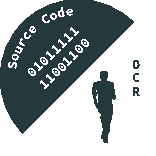
\includegraphics[height=6cm,angle=30]{images/Logo/Logo1.pdf}

\includegraphics[height=4cm,angle=-30]{images/Logo/Logo2.pdf}
 }


Bild (\autoref{fig:bild}).
\begin{figure}[!h]% hier: !hb
	\centering
	\includegraphics[width=.55\textwidth]{images/Logo/logo.eps}
	\caption{Bild}\label{fig:bild}%% anpassen
\end{figure}
 
 
 \section{Links}
 
 PDF öffnen: (\url{images/Logo/Logo-Details.pdf}) 
 
 Video öffnen: \movie[externalviewer]{(video.mov)}{images/Video/video.mov}
 
 Website \footnote{\url{http://bw-ju.de/}}

\section{Tabelle}

% Tab 1
(siehe \autoref{tab:heisetabelle}).
\begin{table}[ht]
\centering
\begin{tabular}{cc}
\toprule 
\textbf{Begriff} & \textbf{Definition}\\
\midrule  
A	&	Text \\
B	&	Text \\ 
C	&	Text \\
D	&	Text \\
E	&	Text \\
F	&	Text \\
\bottomrule
\end{tabular}
\caption{Beschreibung der Tabelle}
\label{tab:heisetabelle}
\end{table}


% Tab 2
\rowcolors{1}{}{grau2}% EIN: oder \showrowcolors o. \hiderowcolors
\begin{table}[h]
\centering
\begin{tabular}{cp{3.5cm}}
\textbf{Begriff} & \textbf{Definition}\\
\hline %\showrowcolors %\hiderowcolors
A	&	Text \\
B	&	Text \\ 
C	&	Text \\
D	&	Text \\
E	&	Text \\
F	&	Mehrzeiliger Text \newline in einer Zelle \\
\end{tabular}
\caption{Beschreibung}
\label{tab:tabelle}
\end{table}
\rowcolors{1}{}{}% AUS

%\newpage
%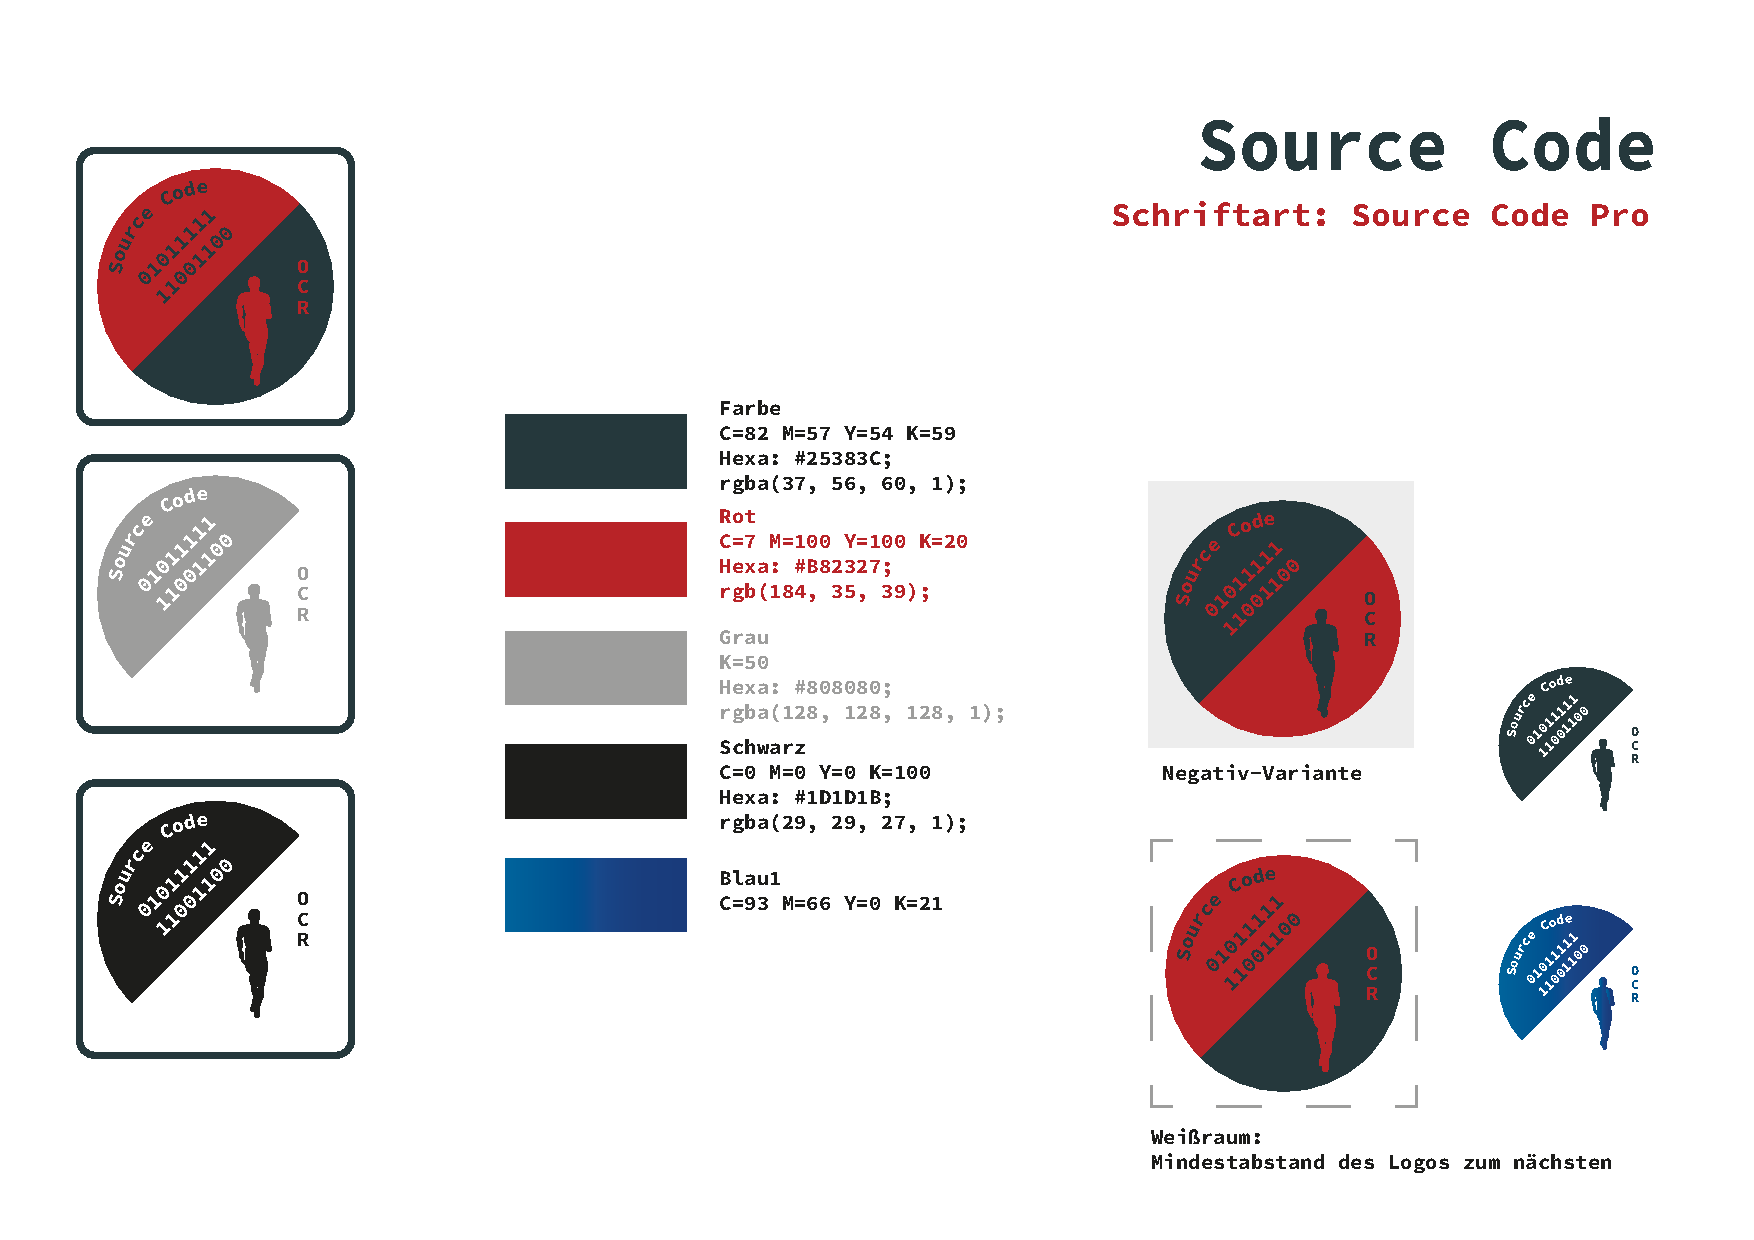
\includepdf[pages=-,landscape]{images/Logo/Logo-Details.pdf}%landscape

\chapter{Spickzettel-Markdown}
%ju 05-Feb-22 Spickzettel-Markdown.tex
\section{Schreiben in Markdown}\label{schreiben-in-markdown}

\begin{enumerate}
\item
  Markdown
\item
  Textauszeichnung -- Was ist wichtig? Tabellen, Bilder, Quellcode,
  Literatur, Links
\item
  Rechtschreibprüfung \footnote{\url{https://languagetoolplus.com/?pk-campaign=addon2-popup-logo}}
\item
  Literatur \footnote{\url{https://www.zotero.org/user/login}}
\end{enumerate}

\section{Markdown -- Latex -- PDF
erstellen}\label{markdown-latex-pdf-erstellen}

\begin{enumerate}
\item
  Markdown > Latex: \verb|$ projekt.sh|
  Script (pandoc)
\item
  Hand-Kopie: \verb|tex\_pandoc/ tex/|
\item
  Referenzen: Links prüfen

  \begin{itemize}
  \item
    Bild %vgl.~(\autoref{fig:}). >
    \verb|(\\autoref\{fig:bild\}).|
  \item
    Tabelle %vgl.~(\autoref{tab:}). >
    \verb|(\\autoref\{tab:tabellen\}).|
  \item
    Kapitel %vgl.~(\autoref{}). >
    \verb|(\\autoref\{sec:zusammenfassung\}).|
  \item
    Code %vgl.~(\autoref{code:}). >
    \verb|(\\autoref\{code:hallowelt\})|.
  \end{itemize}
\item
  Latex > PDF: \verb|$ make| Makefile
  (latexmk)
\end{enumerate}

\section{Quellen}\label{quellen}

Quelle: \textcite{spanner:2019:robotik}

Quelle: \textcite{homofaciens:2018:projekt}

Quelle: \textcite{kofler:2018:hacking}

\lstset{language=Python}% C, TeX, Bash, Python 
\begin{lstlisting}[
	%caption={}, label={code:}%% anpassen
]
Quelle: [@monk:2016:action]
Quelle: [@homofaciens:2018:projekt]
Quelle: [@kofler:2018:hacking]
\end{lstlisting}

\section{Listen}\label{listen}

\textbf{ungeordnete Liste}

\begin{itemize}
\item
  a
\item
  b

  \begin{itemize}
  \item
    BB
  \end{itemize}
\item
  c
\end{itemize}

\lstset{language=Python}% C, TeX, Bash, Python 
\begin{lstlisting}[
	%caption={}, label={code:}%% anpassen
]
- a
- b
    - bb
- c
\end{lstlisting}

\textbf{Sortierte Liste}

\begin{enumerate}
\item
  eins
\item
  zwei
\item
  drei
\end{enumerate}

\lstset{language=Python}% C, TeX, Bash, Python 
\begin{lstlisting}[
	%caption={}, label={code:}%% anpassen
]
1. eins
2. zwei
3. drei
\end{lstlisting}

\textbf{Sortierte Liste}

\begin{enumerate}
\def\labelenumi{\alph{enumi})}
\item
  a
\item
  b
\item
  c
\end{enumerate}

\lstset{language=Python}% C, TeX, Bash, Python 
\begin{lstlisting}[
	%caption={}, label={code:}%% anpassen
]
a) a
b) b
c) c
\end{lstlisting}

\section{Anführungszeichen}\label{anfuehrungszeichen}

>>Anführungszeichen<<

\lstset{language=Python}% C, TeX, Bash, Python 
\begin{lstlisting}[
	%caption={}, label={code:}%% anpassen
]
"Anführungszeichen" 
\end{lstlisting}

\section{Grafik -- Abbildung}\label{grafik-abbildung}

Logo %vgl.~(\autoref{fig:}).

\begin{figure}[!ht]% hier: !ht
\centering
\includegraphics[width=0.3\textwidth]{images/Logo/logo.pdf}
\caption{Logo}
%\label{fig:}%% anpassen
\end{figure}

\lstset{language=Python}% C, TeX, Bash, Python 
\begin{lstlisting}[
	%caption={}, label={code:}%% anpassen
]
![Logo](images/Logo/logo.pdf){width=30%}
\end{lstlisting}

\section{Tabelle}\label{tabelle}

Tabelle-Bsp %vgl.~(\autoref{tab:}).

\begin{table}[!ht]% hier: !ht 
\centering 
	\caption{}% \label{tab:}%% anpassen 
\begin{tabular}{@{}rll@{}}
\hline
\textbf{Nr.} & \textbf{Begriffe} & \textbf{Erklärung} \\
\hline
1 & a1 & a2 \\
2 & b1 & b2 \\
3 & c1 & c2 \\
4 & a1 & a2 \\
\hline
\end{tabular} 
\end{table}

\lstset{language=Python}% C, TeX, Bash, Python 
\begin{lstlisting}[
	%caption={}, label={code:}%% anpassen
]
| **Nr.** | **Begriffe** | **Erklärung** |
| --: | :----- | :---- |
|       1 | a1           | a2            |
|       2 | b1           | b2            |
|       3 | c1           | c2            |
|       4 | a1           | a2            |
\end{lstlisting}

\section{Mathematik}\label{mathematik}

$[ V ] = [ \Omega ] \cdot [ A ]$ o. $U = R \cdot I$ o.
$R = \frac{U}{I}$

\lstset{language=Python}% C, TeX, Bash, Python 
\begin{lstlisting}[
	%caption={}, label={code:}%% anpassen
]
$[ V ] = [ \Omega ] \cdot [ A ]$ o. $U = R \cdot I$ o. $R = \frac{U}{I}$
\end{lstlisting}

$5~cm$, $a \cdot b$, $\cdots$, $\Omega$

$100^\circ\text{C}$

$80~\%$ // in HTML

\lstset{language=Python}% C, TeX, Bash, Python 
\begin{lstlisting}[
	%caption={}, label={code:}%% anpassen
]
$5~cm$, $a \cdot b$, $\cdots$, $\Omega$
$100^\circ\text{C}$  
// ACHTUNG: Prozentzeichen macht Probleme in HTML und Latex 
// Z.B. 80 %
$80~\%$ // in Latex
$80~\%$  // in HTML
\end{lstlisting}

\textbf{Mathematik-Umgebung:}

\begin{align*}
    \sum_{i=1}^5 a_i = a_1 + a_2 + a_3 + a_4 + a_5
\end{align*}

\lstset{language=Python}% C, TeX, Bash, Python 
\begin{lstlisting}[
	%caption={}, label={code:}%% anpassen
]
\begin{align*}
    \sum_{i=1}^5 a_i = a_1 + a_2 + a_3 + a_4 + a_5
\end{align*}
\end{lstlisting}

\section{Texthervorhebung}\label{texthervorhebung}

\textbf{Fett} oder \emph{Kursiv}

\lstset{language=Python}% C, TeX, Bash, Python 
\begin{lstlisting}[
	%caption={}, label={code:}%% anpassen
]
**Fett** oder *Kursiv*
\end{lstlisting}

\section{Code}\label{code}

Hallo Welt %vgl.~(\autoref{code:}).

\lstset{language=Python}% C, TeX, Bash, Python 
\begin{lstlisting}[
	%caption={}, label={code:}%% anpassen
]
// hallowelt.c
#include <stdio.h>
int main(void) {
    printf("Hallo Welt!\n");
    return 0;
}
\end{lstlisting}

\section{Links}\label{links}

\url{https://google.de} oder \href{https://google.de}{Google}

\lstset{language=Python}% C, TeX, Bash, Python 
\begin{lstlisting}[
	%caption={}, label={code:}%% anpassen
]
<https://google.de> oder [Google](https://google.de)
\end{lstlisting}

Fußnote\footnote{\url{https://bw-ju.de/}}

\lstset{language=Python}% C, TeX, Bash, Python 
\begin{lstlisting}[
	%caption={}, label={code:}%% anpassen
]
Fußnote[^1]       

[^1]: <https://bw-ju.de/>
\end{lstlisting}

\section{Absätze}\label{absaetze}

Dies hier ist ein Blindtext zum Testen von Textausgaben. Wer diesen Text
liest, ist selbst schuld. Der Text gibt lediglich den Grauwert der
Schrift an. Ist das wirklich so? Ist es gleichgültig, ob ich schreibe:
>>Dies ist ein Blindtext<< oder >>Huardest gefburn<<? Kjift -
mitnichten! Ein Blindtext bietet mir wichtige Informationen. An ihm
messe ich die Lesbarkeit einer Schrift, ihre Anmutung, wie harmonisch
die Figuren zueinander stehen und prüfe, wie breit oder schmal sie
läuft. Ein Blindtext sollte möglichst viele verschiedene Buchstaben
enthalten und in der Originalsprache gesetzt sein. Er muss keinen Sinn
ergeben, sollte aber lesbar sein.

Fremdsprachige Texte wie >>Lorem ipsum<< dienen nicht dem eigentlichen
Zweck, da sie eine falsche Anmutung vermitteln.


%%%%%%%%%%%%%%%%%%%%%%%%%%%%%%%%%%%%%%%%%%%%%%%%%%

% archiv/

%\chapter{Pics-files}
%% ---------------------------------------------
% Alle Abbildungen 'images/' in Latex speichern 
%     * 'archiv/Pics-files.tex' 
%     * Bildgröße: 0.80/1 
% ju 20-Feb-2022 Pics-files.tex
% ---------------------------------------------
%

%\chapter{Quellcode-files}
%% ---------------------------------
% Quellcode 'code/' in Latex speichern. 
% 'archiv/Quellcode-files.tex' 
% HTML, Python, Bash, C, C++, TeX 
% ju 20-Feb-2022 Quellcode-files.tex
% ---------------------------------
%

\section{Python_keywords}

%Python_keywords.py (\autoref{code:Python_keywords-1}).% Referenz
%
\lstset{language=Python}% HTML, Python, Bash, C, C++, TeX
\lstinputlisting[% anpassen
    caption={Quellcode in Python: Python_keywords.py}, %label={code:Python_keywords-1}
]{code/Python_keywords.py}% file

\newpage


%%%%%%%%%%%%%%%%%%%%%%%%%%%%%%%%%%%%%%%%%%%%%%%%%%

% Tabellen/

%\chapter{PDFs}
%% ju 28-Nov-2021 PDFs.tex 

\chapter{PDF}% book, print anpassen








%%%%%%%%%%%%%%%%%%%%%%%%%%%%%%%%%%%%%%%%%%%%%%%%%%

% content/beispiele/tex/

%\chapter{Aufbau-der-Arbeit}
%%\chapter{Aufbau der Arbeit}

Jede Arbeit besteht in der Regel aus einer \textbf{Problemstellung}, einem \textbf{definitorischen Abschnitt}, der eigentlichen \textbf{Behandlung der Problemstellung} sowie einer \textbf{Zusammenfassung der zentralen Ergebnisse}.

\begin{description}

	\item[Einleitung] Im Zentrum des erstens Teils stehen die Darstellung des Themas der Arbeit und die genaue Auflistung der Fragestellungen (Wieso ist das Thema relevant?). Ebenso sollten schon einzelne Aspekte des Problems herausgearbeitet werden. Dabei ist es hilfreich, die zentralen Fragen aufzulisten, die im Rahmen der Arbeit beantwortet werden sollen.
	
	Außerdem sollte ein knapper Überblick gegeben werden, in welchen Schritten die Problembehandlung erfolgt: Hinführung zum Thema, Herleitung und Ausformulierung der Fragestellung, Abgrenzung des Themas (Angabe von Aspekten, die zum Thema gehören, aber ausgeklammert werden) und Aufbau der Arbeit (Begründung der Gliederung).
	
	\item[Grundlagen (definitorischer Teil)] Im zweiten Teil sollen zentrale Begriffe definiert und eingeordnet werden. Es geht dabei nicht darum, Definitionen aus Lexika zu suchen; stattdessen sollten problemorientierte Definitionen verwendet werden. Häufig können einzelne Begriffe unterschiedlich weit oder eng definiert werden, sodass auch eine Diskussion unterschiedlicher Definitionsansätze hilfreich sein kann, bevor eine für die weitere Arbeit verbindliche Definition gewählt wird. Zudem sollte ein Überblick über die in der Literatur vorhandenen Methoden bzw. Lösungsansätze, der aktuelle Stand der Technik und verwandte Arbeiten gegeben werden.
	
	\item[Hauptteil] Im Hauptteil der Arbeit (der in der Gliederung selbstverständlich nicht so zu benennen ist\ldots) erfolgt die eigentliche eigentliche Auseinandersetzung mit der Problemstellung. In diesem Teil kommt es darauf an, nicht nur Lehrbuchwissen zusammenzutragen, sondern die Problemstellung reflektiert zu bearbeiteten. Aussagen sollten durch herangezogene Literatur gestützt und belegt werden. Bitte darauf achten, in logischen, nachvollziehbaren Schritten vorzugehen.
	
	\item[Schlussbetrachtung] Die Antwort auf die in der Problemstellung aufgeworfenen Fragen soll kurz und prägnant zusammengefasst werden. Ebenso sollte ein Ausblick auf offen gebliebene Fragen sowie auf interessante Fragestellungen, die sich aus der Arbeit ergeben, gegeben werden. Eine kritische Betrachtung der eigenen Arbeit ist an dieser Stelle ebenfalls sinnvoll.

\end{description}

\noindent
Eine Sammlung unserer Tipps für das Schreiben von Ausarbeitungen befindet sich online unter \url{https://www.dcl.hpi.uni-potsdam.de/media/theses/}.

%\chapter{LaTeX-Beispiel-beamer}
%% ju 23-Jul-21
\section*{Einleitung}

\emph{Sonderzeichen}  wie <<\& oder \%>> müssen mit einem Backslash \verb|\& oder \%| maskiert werden, 
damit sie von LaTeX nicht als Befehle missverstanden werden.


\emph{Website} \footnote{\url{https://golatex.de/wiki/Hauptseite}} \verb|\footnote{\url{https://golatex.de/wiki/Hauptseite}}| 

\emph{PDF Datei einbinden} \verb|\includepdf[landscape=false]{images/logo.eps}| 
\includepdf[landscape=false]{images/logo.eps} 

\clearpage
\subsection*{Stand der Forschung}

Während die traditionelle Latexproduktion bereits hinreichend erforscht ist (\autoref{fig:latex}) \\
\verb|(\autoref{fig:latex})|, bleibt das wissenschaftliche Verständnis elektronischer Verarbeitungsprozesse dieses 
vielseitigen Materials weiterhin lückenhaft. 


\begin{figure}[!ht]% hier: !ht
	\centering
	\includegraphics[width=0.25\textwidth]{images/logo.eps}
	\caption{Traditionelle Latexproduktion}\label{fig:latex}%
\end{figure}

\lstset{language=TeX}% C, TeX, Bash, Python 
\begin{lstlisting}[
	%caption={}, label={code:}%% anpassen
]
% Optionen
scale = Wert, Vergrösserungsfaktor
width/height = Wert für die Einstellung der Breite/Höhe
angle = Wert, Winkel (in Grad)
b = bottom - Seitenende 
t = top - Seitenanfang
h = here
p = page - komplette Seite  
% Abbildung
\begin{figure}[!ht]% hier: !ht
	\centering
	\includegraphics[width=0.25\textwidth]{images/logo.eps}
	\caption{Traditionelle Latexproduktion}\label{fig:latex}%
\end{figure}
\end{lstlisting}


\clearpage
\section*{Methodik}

Unter Zuhilfenahme der Formeln \autoref{eq:ekin} \verb|\autoref{eq:ekin}| und \autoref{eq:impuls} \verb|\autoref{eq:impuls}| werden wir 
diese Forschungslücke schließen.  
$E_{kin}$ \verb|$E_{kin}$| ist die kinetische Energie, $m$ \verb|$m$| die Masse und $\vec{v}$ \verb|$\vec{v}$| die Geschwindigkeit.

Wurzel $\sqrt{2}$ \verb|$\sqrt{2}$|

Bruch $\frac{\text{Zähler}}{\text{Nenner}}$ \verb|$\frac{\text{Zähler}}{\text{Nenner}}$|

\begin{equation}
	\label{eq:ekin}% 
	\sum E_{kin} = \sum E'_{kin}
\end{equation}

\begin{equation}
	\label{eq:impuls}% 
	\vec{v_1} - \vec{v_1'} = \frac{m_2}{m_1} (\vec{v_2'} - \vec{v_2})
\end{equation}

\lstset{language=TeX}% C, TeX, Bash, Python 
\begin{lstlisting}[
	%caption={}, label={code:}%% anpassen
]
% Mathe
\begin{equation}
	\label{eq:ekin}% 
	\sum E_{kin} = \sum E'_{kin}
\end{equation}
\end{lstlisting}


\clearpage
\section*{Ausblick}

Daraus ergeben sich gemäß (\autoref{tab:schritte}) \verb|(\autoref{tab:schritte})| folgende nächste Schritte, 
deren sequenzielle Ausführung von essenzieller Bedeutung ist.

\begin{table}[!ht]% hier: !ht
	\centering
	\begin{tabular}{@{}cl@{}}% lcr
		\toprule
		\textbf{Nr.} & \textbf{Vorgehen} \\
		\midrule
		1 & Aktuellen Forschungsstand recherchieren \\
		2 & Methoden entwickeln \\
		3 & Schlussfolgerung aufstellen \\
		\bottomrule
	\end{tabular}
	\caption{Nächste Schritte}\label{tab:schritte}
\end{table}

\clearpage
\lstset{language=TeX}% C, TeX, Bash, Python 
\begin{lstlisting}[
	%caption={}, label={code:}%% anpassen
]
% Tabelle
\begin{table}[!ht]% hier: !ht
	\centering
	\begin{tabular}{@{}cl@{}}% lcr
		\toprule
		\textbf{Nr.} & \textbf{Vorgehen} \\
		\midrule
		1 & Aktuellen Forschungsstand recherchieren \\
		2 & Methoden entwickeln \\
		3 & Schlussfolgerung aufstellen \\
		\bottomrule
	\end{tabular}
	\caption{Nächste Schritte}\label{tab:schritte}
\end{table}
\end{lstlisting}
%\chapter{Latex-install-Ubuntu}
%% letztes Update: 27-Jul-20
Quelle: Dr.~Uwe Ziegenhagen -- Anleitung zur TEX Live Installation

\section{TEX Live Download}\label{tex-live-download}

Download \footnote{\url{http://mirror.ctan.org/systems/texlive/tlnet}}

Download-texlive vgl.~(\autoref{code:Download-texlive}).

\lstset{language=C}% C, TeX, Bash, Python 
\begin{lstlisting}[%% anpassen
caption={Download-texlive},label={code:Download-texlive}
]
cd Downloads
tar xvfz install-tl-unx.tar.gz
cd install-tl-20200114
perl install-tl
perl install-tl -gui
\end{lstlisting}

\section{TeX Version}\label{tex-version}

tex --version

\section{TEX Live Installation}\label{tex-live-installation}

Install-texlive vgl.~(\autoref{code:Install-texlive}).

\lstset{language=C}% C, TeX, Bash, Python 
\begin{lstlisting}[%% anpassen
caption={Install-texlive},label={code:Install-texlive}
]
sudo apt install texlive texlive-latex-recommended texlive-fonts-recommended \
    texlive-latex-base texlive-base texlive-latex-extra texlive-lang-german

# Verbesserte Schriftarten bei T1-Kodierung
sudo apt-get install cm-super 
\end{lstlisting}

\section{Umgebungsvariablen für
Unix}\label{umgebungsvariablen-fuer-unix}

Umgebungsvariable vgl.~(\autoref{code:Umgebungsvariable}).

\lstset{language=C}% C, TeX, Bash, Python 
\begin{lstlisting}[%% anpassen
caption={Umgebungsvariable},label={code:Umgebungsvariable}
]
vi ~/.profile
# Datei 
PATH=/usr/local/texlive/2019/bin/x86_64-linux:$PATH; export PATH
MANPATH=/usr/local/texlive/2019/texmf-dist/doc/man:$MANPATH; export MANPATH
INFOPATH=/usr/local/texlive/2019/texmf-dist/doc/info:$INFOPATH; export INFOPATH

sudo vi /etc/manpath.config
# Datei 
MANPATH_MAP /usr/local/texlive/2019/bin/x86_64-linux \
  /usr/local/texlive/2019/texmf-dist/doc/man  
\end{lstlisting}

%\chapter{Mathe-Aufgaben}
%
\textbf{Aufgabe 1:} \enspace Jasmin hat ihre Freunde Nico, Laura und Anna zum Geburtstag eingeladen. Nico will nicht kommen, wenn Laura nicht kommt. Laura und Anna kommen beide oder kommen beide nicht. Aber Anna sagt: >>Wenn Nico und Laura beide nicht kommen, dann komme ich.<< Wer von den dreien wird unter diesen Bedingungen tatsächlich zum Geburtstag erscheinen?


\textbf{Aufgabe 2:} \enspace In der Anwaltsserie >>Suits<< (Staffel 4, Folge 1) kommt es zu Folgendem Gespräch zwischen Mike und seiner Sekräterin Amy.


\begin{enumerate}[label={\protect\ding{\value*}},start=192]
    \item Amy: >>Und wie lief dein Treffen mit dem geheimnisvollen Harvey Specter?<<
    \item Mike: >>Ein Arsch zu sein macht einen nicht geheimnisvoll.<<
    \item Amy: >>Na dann bist du ja ein ganz offenes Buch.<<
\end{enumerate}

Untersuchen Sie das Gespräch aussagenlogisch und prüfen Sie den Wahrheitswert von Amys Aussage.


\textbf{Aufgabe 3:} \enspace Formalisieren Sie die folgenden Aussagen und verneinen Sie sie anschließend (ohne das Wort nicht davor zu setzen) und übersetzen Sie wieder in Umgangssprache:

\begin{enumerate}[label=(\alph*)]
    \item Volksmund: >>Bei Nacht sind alle Katzen grau.<<
    \item Plakatwerbung: >>Wenn einer hochguckt, dann gucken alle.<<
    \item Gorbatschov: >>Wer zu spät kommt, den bestraft das Leben.<<
\end{enumerate}

\textbf{Aufgabe 4:} \enspace Wurzel

\begin{multicols}{3}
    \begin{enumerate}[label=(\alph*)]
        \item $\sqrt{169}$
        \item $\sqrt{0,36}$
        \item $\frac{\sqrt{45}}{\sqrt{80}}$
        \item $\sqrt{32}$
        \item $\sqrt{2}$
        \item $\sqrt{1,44}$
        \item $\sqrt{\frac{75}{12}}$
    \end{enumerate}
\end{multicols}
%\chapter{Mathe-Latex}
%\section{\textbf{Text Unterstreichen}}
    \underline{wichtiger Text} und \emph{kursiver Text} und \textbf{fetter Text}

 
\section{\textsc{Kapitaelchen}}  
    Text in Grossbuchstaben setzen durch \LaTeX
    \begin{itemize} % \item[] avoids bullet
        \item[] Einen längeren Satz\\ einrücken.
    \end{itemize}

\section{Vor- und Nachteile}
    \begin{tabular}[h]{ll}
        {\textbf{Vorteile}}   &  {\textbf{Nachteile}} \\
        Argument 1            &  Argument 2 \\
        Argument A            &  Argument B \\
    \end{tabular} 

\section{Summe}
    \begin{tabular}[h]{clrr}
        & Betrag &               &  $1.000,00$ \\
    $-$ & Skonto & $2\%$         &     $20,00$ \\
        \hline
    $=$ & $\sum$ &               &    $980,00$  
    \end{tabular} 
    
\section{Division Zinsen}
    $
        \frac{\text{ Betrag } \cdot \text{ Prozentsatz } \cdot \text{ Zeit } }{100 \cdot \text{ Zeitgröße }} 
        = \frac{12.597,90 \cdot 12 \cdot 20 \text{ T } }{100 \cdot 360} 
        = 83,99 \text{ \euro }
    $

    \begin{align*}
        \frac{\text{ Betrag } \cdot \text{ Prozentsatz } \cdot \text{ Zeit } }{100 \cdot \text{ Zeitgröße }} 
        = \frac{12.597,90 \cdot 12 \cdot 20 \text{ T } }{100 \cdot 360} 
        = 83,99 \text{ \euro }
    \end{align*} 

\section{Tabelle 2}
    \begin{table}[!ht]% hier: !ht 
        \begin{tabular}{@{}lcr@{}}
        \toprule 
        \textbf{Großbuchstaben} & \textbf{Kleinbuchstaben} & \textbf{Name}\\
        \midrule
        21 \euro & 22000 & 230.000 \\
        $31$ \euro & $32000$ & $330.000$ \\
        \bottomrule
        \end{tabular}
    \end{table}

\section{Checkliste}
    Meine Liste
    \begin{itemize} \itemsep -2pt  % reduce space between items
        \item[$\Box$]   Punkt 1
        \item[$\Box$]   Aufgabe 2 
    \end{itemize}

    \begin{itemize}[label=\checkmark] \itemsep -2pt
        \item Check 1
        \item Check 2   
    \end{itemize}

\section{\textcolor{rot5}{Nenne 4x Lerzielstufen (Taxonomien)}}
    \begin{enumerate}[label={\protect\ding{\value*}},start=192]
        \item Reproduktion
        \item Reorganisieren
        \item Transfer
        \item Kreativ
    \end{enumerate}

\section{Wurzel berechnen}
    \begin{multicols}{3}
        \begin{enumerate}[label=(\alph*)]
            \item $\sqrt{169}$
            \item $\sqrt{0,36}$
            \item $\frac{\sqrt{45}}{\sqrt{80}}$
        \end{enumerate}
    \end{multicols}

\section{Aufgabe Logik}
    Formalisieren Sie die folgenden Aussagen und verneinen Sie sie anschließend (ohne das Wort nicht davor zu setzen) und übersetzen Sie wieder in Umgangssprache:

    \begin{enumerate}[label=(\alph*)]
        \item Volksmund: >>Bei Nacht sind alle Katzen grau.<<
        \item Plakatwerbung: >>Wenn einer hochguckt, dann gucken alle.<<
        \item Gorbatschov: >>Wer zu spät kommt, den bestraft das Leben.<<
    \end{enumerate}

\section{Quotientenregel}
    \begin{itemize} % \item[] ohne bullet
        \item[] $\left(\frac{u}{v}\right)^{\prime} = \frac{u^{\prime} \cdot v-u \cdot v^{\prime}}{v^{2}}$
        
        \item[] $\frac{\text{ Ableiten } \cdot \text{ Stehen lassen } - \text{ Stehen lassen } \cdot \text{ Ableiten }}{\text{ Nenner}^2}$
    \end{itemize}

    
\section{Logarithmus}
    \begin{align}
        ln(a \cdot b)   &= ln(a) + ln(b) \\
        ln(\frac{a}{b}) &= ln(a) - ln(b) \\
        ln(a^b)         &= b \cdot ln(a)
    \end{align}

    \newpage
\section{\LaTeX - Assistent}
    Formeleditor~\footnote{\url{https://www.matheretter.de/rechner/latex}}
    \begin{align}
        \text{ Matrix }       &= \begin{pmatrix} a & b \\ c & d \end{pmatrix} \\
        \text{ Vektor }       &= \begin{pmatrix} x\\y \end{pmatrix} \\
        \text{ Vektorbuchstabe } &= \vec{x} \\
        \text{ Wurzel }       &= \sqrt[n]{a} \text{ Potenz } a^{b} \\
        \text{ Bruch }        &= \frac{a}{b} \\
        \text{ Log }          &= \log_{b}{a} \\
        \text{ Summe }        &= \sum \limits_{n=0}^{\infty} \\
        \text{ Index }        &= x_{1,2} \\
        \text{ Klammern }     &= \left\{x, y\right\} \\
        \text{ Alphabet kl. } &= +\\%α β γ δ ε ζ η θ ι κ λ μ ν ξ ο π ρ σ τ υ φ χ ψ ω \\
        \text{ Alphabet gr. } &= +\\%Α Β Γ Δ Ε Ζ Η Θ Ι Κ Λ Μ Ν Ξ Ο Π Ρ Σ Τ Υ Φ Χ Ψ Ω \\
        \text{ Element }      &= \in \notin \sum \quad \prod \quad () \quad \to \quad \infty\\
        \text{ Mengen }       &= \mathbb{N} \mathbb{Z} \mathbb{Q} \mathbb{R} \mathbb{I} \mathbb{C} \mathbb{L} \\
        \text{ Relation }     &= < > \geq \leq \neq \subset \subseteq \approx \in \supset \supseteq \notin \\
        \text{ Pfeile }       &= +\\%\rightarrow \leftarrow \Longleftrightarrow \Longrightarrow \Longleftarrow \\
    \end{align}

\section{Formeln in einer Zeile}
    $
        u = \bar{u} + \epsilon \cdot u_1 \quad
        v = \bar{v} + \epsilon \cdot v_1 \quad
        w = \bar{w} + \epsilon \cdot w_1 \quad
    $

    $
        \left( \begin{array}{rrr}
            1 & 0 & 0 \\                                              
            0 & 1 & 0 \\
            0 & 0 & 1 \\                                              
        \end{array}\right)
    $

\section{Sonderzeichen}
    \textbackslash \{...\} \$ \& \# \textdegree \^{} \_ \textasciitilde \%

\section{Währungszeichen}
    \euro 100 \textdollar 100 \textsterling 100 $1.000,00 \text{ \euro }$ 1.000,00 \euro

\section{Leerzeichen}
\begin{itemize} % \item[] avoids bullet
    \item[] [a\,b] ($0.16667em$)
    \item[] [a\:b] ($0.2222em$)
    \item[] [a\enspace b] ($0.5em$)
    \item[] [a\quad b] ($1em$)
    \item[] [a\hspace{5em} b] (5em)
\end{itemize}

\newpage
\section{Griechisches Alphabet}
    \begin{table}[!ht]% hier: !ht 
        \begin{tabular}{@{}ccl@{}}
        \toprule 
        \textbf{Großbuchstaben} & \textbf{Kleinbuchstaben} & \textbf{Name}\\
        \midrule
        A & $\alpha$ & Alpha\\
        B & $\beta$ & Beta\\
        $\Gamma$ & $\gamma$ & Gamma \\
        $\Delta$ & $\delta$ & Delta\\
        E & $\epsilon$, $\varepsilon$ & Epsilon\\
        Z & $\zeta$ & Zeta\\
        H & $\eta$ & Eta\\
        $\Theta$ & $\theta$, $\vartheta$ & Theta\\
        I & $\iota$ & Iota\\
        K & $\kappa$, $\varkappa$ & Kappa\\
        $\Lambda$ & $\lambda$ & Lambda\\
        M & $\mu$ & My\\
        N & $\nu$ & Ny\\
        $\Xi$ & $\xi$ & Xi\\
        O & o & Omikron\\
        $\Pi$ & $\pi$, $\varpi$ & Pi\\
        P & $\rho$, $\varrho$ & Rho\\
        $\Sigma$ & $\sigma$, $\varsigma$ & Sigma\\
        T & $\tau$ & Tau\\
        Y & $\upsilon$ & Ypsilon\\
        $\Phi$ & $\phi$, $\varphi$ & Phi\\
        X & $\chi$ & Chi\\
        $\Psi$ & $\psi$ & Psi\\
        $\Omega$ & $\omega$ & Omega\\
        \bottomrule
        \end{tabular}
    \end{table}

\section{Tabelle 3}
    Tabellengenerator~\footnote{\url{https://www.tablesgenerator.com/}} 
    und Rechner~\footnote{\url{https://www.matheretter.de/rechner/latex}}

    \begin{multicols}{2}
        \begin{tabular}[h]{ll|l}
            &  A     & B     \\ 
        \hline
        1)* &  $a_1$ & $b_1$ \\
        2)  &  $a_2$ & $b_2$ \\
        3)  &  $a_3$ & $b_3$ 
        \end{tabular}
        
        \columnbreak% Spalte
        *Beachte: $\sqrt[n]{x} = x^\frac{1}{n}$       
    \end{multicols}

\section{Tabelle und Grafik}
    \begin{multicols}{2}
        \begin{tabular}[h]{l|c|r}
            Spalte 1 & Spalte 2 & Spalte 3 \\
            \hline
            heise & tipps & tricks \\
        \end{tabular}    

        \columnbreak% Spalte

        \includegraphics[width=2.0cm]{images/logo.eps}% Logo   
    \end{multicols}  

\newpage
\section{Farben}
    \begin{testcolors}[rgb,cmyk,HTML,gray]
        \testcolor{black}
        \testcolor{white}
        \testcolor{darkgray}
        \testcolor{gray}
        \testcolor{lightgray}
        \testcolor{red}
        \testcolor{green}
        \testcolor{blue}
        \testcolor{cyan}
        \testcolor{magenta}
        \testcolor{yellow}
        \testcolor{brown}
        \testcolor{lime}
        \testcolor{olive}
        \testcolor{orange}
        \testcolor{pink}
        \testcolor{purple}
        \testcolor{teal}
        \testcolor{violet}
        \testcolor{rot5}
        \testcolor{blau5}  
        \testcolor{grau2}    
        \testcolor{orange}                       
    \end{testcolors}
    
\section{Farbenfolgen}
    \definecolorseries{test}{rgb}{step}[rgb]{.95,.85,.55}{.17,.47,.37}
    \definecolorseries{test}{hsb}{step}[hsb]{.575,1,1}{.11,-.05,0}
    \definecolorseries{test}{rgb}{grad}[rgb]{.95,.85,.55}{3,11,17}
    \definecolorseries{test}{hsb}{grad}[hsb]{.575,1,1}{.987,-.234,0}
    \definecolorseries{test}{rgb}{last}[rgb]{.95,.85,.55}[rgb]{.05,.15,.55}
    \definecolorseries{test}{hsb}{last}[hsb]{.575,1,1}[hsb]{-.425,.15,1}
    \definecolorseries{test}{rgb}{last}{red!50}{blue}
    \definecolorseries{test}{hsb}{last}{yellow!50}{black}
    \definecolorseries{test}{cmy}{last}{orange!50}{green}

    \resetcolorseries[12]{test}
    \rowcolors[\hline]{1}{test!!+}{test!!+}
    \setlength{\tabcolsep}{5mm} % Abstände zwischen den Spalten
    \begin{tabular}[h]{c||c||c||c||c||c||c||c||c||c}
        $S_1$ & $S_2$ & $G_1$ & $G_2$ & $L_1$ & $L_2$ & $L_3$ & $L_4$ & $L_5$ \\
        \hline \hline
        \number\rownum & \number\rownum & \number\rownum & \number\rownum & \number\rownum & \number\rownum & \number\rownum & \number\rownum & \number\rownum \\
        \number\rownum & \number\rownum & \number\rownum & \number\rownum & \number\rownum & \number\rownum & \number\rownum & \number\rownum & \number\rownum \\
        \number\rownum & \number\rownum & \number\rownum & \number\rownum & \number\rownum & \number\rownum & \number\rownum & \number\rownum & \number\rownum \\
        \number\rownum & \number\rownum & \number\rownum & \number\rownum & \number\rownum & \number\rownum & \number\rownum & \number\rownum & \number\rownum \\
        \number\rownum & \number\rownum & \number\rownum & \number\rownum & \number\rownum & \number\rownum & \number\rownum & \number\rownum & \number\rownum \\
        \number\rownum & \number\rownum & \number\rownum & \number\rownum & \number\rownum & \number\rownum & \number\rownum & \number\rownum & \number\rownum \\
        \number\rownum & \number\rownum & \number\rownum & \number\rownum & \number\rownum & \number\rownum & \number\rownum & \number\rownum & \number\rownum \\
        \number\rownum & \number\rownum & \number\rownum & \number\rownum & \number\rownum & \number\rownum & \number\rownum & \number\rownum & \number\rownum \\
        \number\rownum & \number\rownum & \number\rownum & \number\rownum & \number\rownum & \number\rownum & \number\rownum & \number\rownum & \number\rownum \\
        \number\rownum & \number\rownum & \number\rownum & \number\rownum & \number\rownum & \number\rownum & \number\rownum & \number\rownum & \number\rownum \\
        \number\rownum & \number\rownum & \number\rownum & \number\rownum & \number\rownum & \number\rownum & \number\rownum & \number\rownum & \number\rownum \\
        \number\rownum & \number\rownum & \number\rownum & \number\rownum & \number\rownum & \number\rownum & \number\rownum & \number\rownum & \number\rownum \\
        \number\rownum & \number\rownum & \number\rownum & \number\rownum & \number\rownum & \number\rownum & \number\rownum & \number\rownum & \number\rownum \\
        \number\rownum & \number\rownum & \number\rownum & \number\rownum & \number\rownum & \number\rownum & \number\rownum & \number\rownum & \number\rownum \\
        \number\rownum & \number\rownum & \number\rownum & \number\rownum & \number\rownum & \number\rownum & \number\rownum & \number\rownum & \number\rownum \\ 
    \end{tabular}
%\chapter{README}
%\chapter{Readme}\label{readme}

Erstellt Webseiten \& Latex-Files mit Markdown und Pandoc. Projekt wurde
getestet unter >>iMac<<

\section{Kurzbefehle}\label{kurzbefehle}

\textbf{Terminal} öffnen

\lstset{language=Bash}% C, TeX, Bash, Python 
\begin{lstlisting}[
	%caption={}, label={code:}%% anpassen
]
# Schreiben in Markdown, Illustrator für Vektorgrafiken und Excel für Tabellen

./projekt.sh  # Schritt 2, 3, 5
##########################################################
    0) Projekt aufräumen
    1) Projekt erstellen
    2) Markdown in (tex, html5) + sed (Suchen/Ersetzen)
    3) Kapitel erstellen + Scripte ausführen
    4) Fotos optimieren (Web, Latex)
    5) www + index.html
    6) git init
    7) git status + git log
    8) Git-Version erstellen
    9) Backup + Archiv erstellen
##########################################################

# PDF erstellen
make distclean
make
make clean

# Git Version
git add .
git commit -a
git push

# Backup
./projekt.sh  # Schritt 9
\end{lstlisting}

\section{Software}\label{software}

\begin{itemize}
\item
  Git Bash\footnote{\url{https://git-scm.com/downloads}}
\item
  Git-Repository klonen\footnote{\url{https://github.com/ju1-eu/Notizen-TeX-Web-iMac.git}}
\item
  Texlive (Latex)\footnote{\url{https://www.tug.org/texlive/}}
\item
  Pandoc (Dokumentenkonverter)\footnote{\url{https://pandoc.org/installing.html}}
\item
  Imagemagick (Bildbearbeitung)\footnote{\url{https://imagemagick.org/script/download.php}}
\item
  Editor Visual Studio Code\footnote{\url{https://code.visualstudio.com/}}
\item
  Editor Atom\footnote{\url{https://atom.io/}}
\item
  Editor Notepad++\footnote{\url{https://notepad-plus-plus.org/downloads/}}
\item
  TeXstudio (Latexeditor)\footnote{\url{https://www.texstudio.org/}}
\item
  Tablesgenerator (Latex / Markdown)\footnote{\url{https://www.tablesgenerator.com/latex_tables}}
\item
  hpi-dokumentvorlagen-latex (Hasso-Plattner-Institut (HPI)
  Potsdam)\footnote{\url{https://osm.hpi.de/theses/tipps\#dokumentvorlagen-latex}}
\item
  Zotero (Literaturverwaltung)\footnote{\url{http://www.zotero.org/}}
\item
  WordPress\footnote{\url{https://de.wordpress.org/download/}}
\item
  XAMPP Apache + Maria DB + PHP\footnote{\url{https://www.apachefriends.org/de/index.html}}
\item
  FileZilla\footnote{\url{https://filezilla-project.org/}}
\item
  VM VirtualBox\footnote{\url{https://www.virtualbox.org/}}
\item
  Ubuntu (Desktop / Server)\footnote{\url{https://ubuntu.com/download}}
\item
  WordPress-Themes\footnote{\url{https://de.wordpress.org/themes/}}
\item
  themecheck (WordPress-Themes)\footnote{\url{https://themecheck.info/}}
\item
  ghostscript Z.~B. EPS in PDF\footnote{\url{https://www.ghostscript.com/}}
\end{itemize}

\section{Erste Schritte}\label{erste-schritte}

\textbf{Files anpassen:}

\begin{enumerate}
\item
  \verb|scripteBash/sed.sh|

  \begin{itemize}
  \item
    codelanguage:
    \verb|HTML5, Python, Bash, C, C++, TeX|
  \item
    CMS Server Pfad: \verb|https://bw-ju.de/\#|
  \item
    Bildformat: SVG, PNG, JPG, WebP
  \end{itemize}
\item
  \verb|scripteBash/gitversionieren.sh|

  \begin{itemize}
  \item
    >>/Volumes/usb-daten/meineNotizen/repository/notizen-iMac<<
  \end{itemize}
\item
  \verb|projekt.sh|

  \begin{itemize}
  \item
    THEMA=>>Notizen-TeX-Web-iMac<<
  \item
    >>/Volumes/usb-daten/meineNotizen/backup/notizen-iMac<<
  \item
    >>/Volumes/usb-daten/meineNotizen/archiv/notizen-iMac<<
  \end{itemize}
\item
  \verb|content/metadata.tex|

  \begin{itemize}
  \item
    Datum, Titel, Autor
  \end{itemize}
\item
  \verb|content/titelpage.tex|

  \begin{itemize}
  \item
    >>Grafiken/logo.eps<<
  \end{itemize}
\end{enumerate}

\textbf{Markdown-Files erstellen}

\begin{enumerate}
\item
  Erstelle eine Datei >>neu.md<< im Ordner >>md/<<

  \begin{itemize}
  \item
    Bilder nach \verb|images/| kopieren
  \item
    Vektorgrafiken nach \verb|Grafiken/| kopieren
  \end{itemize}
\item
  Script ausführen: \verb|projekt.sh|
\end{enumerate}

\textbf{Terminal} öffnen

\lstset{language=Bash}% C, TeX, Bash, Python 
\begin{lstlisting}[
	%caption={}, label={code:}%% anpassen
]
$ ./projekt.sh

  0) Projekt aufräumen
  1) Projekt erstellen
  2) Markdown in (tex, html5) + sed (Suchen/Ersetzen)
  3) Kapitel erstellen + Scripte ausführen
  4) Fotos optimieren (Web, Latex)
  5) www + index.html
  6) git init
  7) git status + git log
  8) Git-Version erstellen
  9) Backup + Archiv erstellen
 10) Beenden?

 Eingabe Zahl >_
\end{lstlisting}

\begin{enumerate}
\setcounter{enumi}{2}
\item
  Latex-PDFs erstellen: \verb|make|
\end{enumerate}

\lstset{language=Bash}% C, TeX, Bash, Python 
\begin{lstlisting}[
	%caption={}, label={code:}%% anpassen
]
$ make
$ make clean
$ make distclean
\end{lstlisting}

\begin{enumerate}
\setcounter{enumi}{3}
\item
  Repository auf Github erstellen
\end{enumerate}

\section{Git-Repository erstellen --
klonen}\label{git-repository-erstellen-klonen}

GitHub's Maximum File size of \textbf{50 MB}

\textbf{Repository auf Github erstellen}

\lstset{language=Bash}% C, TeX, Bash, Python 
\begin{lstlisting}[
	%caption={}, label={code:}%% anpassen
]
# HTTPS oder SSH
HTTPS: https://github.com/ju1-eu/Notizen-TeX-Web-iMac.git
SSH: git@github.com:ju1-eu/Notizen-TeX-Web-iMac.git

# create a new repository 
echo "# README" >> README.md
# iMac Warnung 
# git config --global init.defaultBranch master
git init
git add .
git commit -m "git init"
                
# or push an existing repository 
git remote add origin https://github.com/ju1-eu/Notizen-TeX-Web-iMac.git
git push -u origin master
\end{lstlisting}

\textbf{Git-Repository klonen}

\lstset{language=Bash}% C, TeX, Bash, Python 
\begin{lstlisting}[
	%caption={}, label={code:}%% anpassen
]
git clone https://github.com/ju1-eu/Notizen-TeX-Web-iMac.git
\end{lstlisting}

\section{Script Beschreibung}\label{script-beschreibung}

\verb|$ ./projekt.sh|

\begin{enumerate}
\item
  Projekt erstellen

  \begin{itemize}
  \item
    Verzeichnis erstellen, wenn nicht vorhanden
  \end{itemize}
\item
  Markdown in \verb|*.tex und *.html|

  \begin{itemize}
  \item
    Markdown in Latex + HTML5 + WordPress
  \item
    sed > WordPress
  \item
    sed > Latex
  \end{itemize}
\item
  Kapitel erstellen + Scripte ausführen

  \begin{itemize}
  \item
    Alle Abbildungen >>images/<< in Markdown speichern.

    \begin{itemize}
    \item
      >>archiv/input-img.txt<<
    \end{itemize}
  \item
    Latex Kapitel erstellen.

    \begin{itemize}
    \item
      Kopiere >>tex-pandoc/.tex<< nach >>tex/<<
    \item
      >>tex/<< \textbf{Handarbeit\ldots{}} für optimale Ergebnisse!
    \item
      Kopiere >>archiv/inhalt.tex<< nach >>content/<<
    \item
      make -- Latex-PDF erstellen
    \end{itemize}
  \item
    Tabellen als PDFs in Latex einfügen. >>Tabellen/ ?<<
  \item
    Inhalt vom Projektverzeichnis.

    \begin{itemize}
    \item
      >>archiv/Projekt-Inhalt.txt<<
    \end{itemize}
  \item
    Quellcode >>code/<< in Latex speichern.

    \begin{itemize}
    \item
      >>archiv/Quellcode-files.tex<< HTML, Python, Bash, C, C++, TeX
    \end{itemize}
  \item
    Artikel aus den Ordnern erstellen

    \begin{itemize}
    \item
      >>tex/<<
    \item
      >>archiv/<<
    \item
      >>Tabellen/<<
    \item
      >>content/beispiele/tex/<<
    \item
      wird gespeichert in >>Artikel/<<
    \end{itemize}
  \item
    Alle Abbildungen >>images/<< in Latex speichern

    \begin{itemize}
    \item
      >>archiv/Pics-files.tex<<
    \item
      Bildgröße: \verb|width=.80\\textwidth|
    \end{itemize}
  \end{itemize}
\end{enumerate}

\begin{enumerate}
\setcounter{enumi}{3}
\item
  Fotos optimieren (Web, Latex)
\item
  www + index.html

  \begin{itemize}
  \item
    >>html/alle-pics.html<< erstellen
  \item
    >>index.html<< erstellen
  \end{itemize}
\item
  \verb|git init|
\item
  \verb|git status| +
  \verb|git log|
\item
  Git-Version erstellen

  \begin{itemize}
  \item
    \textbf{Pfade} anpassen in
    \verb|gitversionieren.sh|
  \item
    lokales Repository: master
  \item
    Github Repository: origin/master
  \item
    Sicherung Repository: backupUSB/master

    \begin{itemize}
    \item
      >>/Volumes/usb-daten/meineNotizen/repository/notizen-iMac<<
    \end{itemize}
  \end{itemize}
\item
  Sicherung + Archiv erstellen

  \begin{itemize}
  \item
    \textbf{Pfade} anpassen in \verb|projekt.sh|
  \item
    THEMA=>>Notizen-TeX-Web-iMac<<
  \item
    >>/Volumes/usb-daten/meineNotizen/backup/notizen-iMac<<
  \item
    >>/Volumes/usb-daten/meineNotizen/archiv/notizen-iMac<<
  \end{itemize}
\end{enumerate}

%\chapter{Spickzettel-LaTeX}
%% letztes Update: 20-Okt-19
%\chapter{Spickzettel -- \LaTeX}

\section{Quellenangabe}\label{sec:quellenangabe}\index{Quellenangabe}

\verb|\textcite|

Zitat: vgl. \textcite{monk:2016:action} und \textcite{kofler:2017:linux}.

Quelle: \textcite{kofler:2018:hacking}.

Quelle: \textcite[87]{schmidt:2015:klima} und \textcite{schneehage:2018:aktoren}.

vgl. \textcite{zeller:2017:hindernis}, \textcite{marquardt:2018:trainingsplan10km} und \textcite{lauren:2017:fit}.


\section{Referenz und Links}\label{sec:referenzlinks}\index{Referenz}

\begin{itemize}
	\item Link \footnote{\url{https://bw-ju.de/}} \verb|\footnote{\url{}}|
	\item Link \url{https://bw-ju.de/} \verb|\url{}|
	\item Link auf File \url{https://github.com/ju1-eu/dummy-notizenUbuntu-v03/blob/master/README.pdf}
	\item Referenz auf Bild (\autoref{fig:bild}). \verb|(\autoref{fig:}).|
	\item Referenz auf Tabellen (\autoref{tab:tabellen}). \verb|(\autoref{tab:}).|
	\item Referenz auf Kapitel (\autoref{sec:zusammenfassung}). \verb|(\autoref{sec:}).|
 	\item Referenz auf Code (\autoref{code:halloweltex}). \verb|(\autoref{code:}).|
	\item Textfußnote \footnote{Fußnote} \verb|\footnote{}|
\end{itemize}


\section{Quellcode}\index{Quellcode}

Programmiersprache C++ (\autoref{code:halloweltex}).
\lstset{language=C++}% C, TeX, Bash, Python
\lstinputlisting[%% anpassen
caption={Programmiersprache C++},label={code:halloweltex}]
{content/beispiele/code/hallo-c++.cpp}


\LaTeX -Syntax (\autoref{code:latexsyntax}). 
\lstset{language=TeX}% C, TeX, Bash, Python
\begin{lstlisting}[%% anpassen
caption={\LaTeX-Syntax},label={code:latexsyntax}]
% artikel.tex
\documentclass[a4paper, 12pt, fleqn, parskip=half]{scrartcl}
\usepackage[ngerman]{babel}
\usepackage[utf8]{inputenc}
\usepackage{times}
\usepackage{booktabs}
\usepackage{graphicx}
\begin{document}
Hallo Welt!
\end{document}
\end{lstlisting}

\section{Text und Absatz}\index{Absatz}

Dies ist ein Typoblindtext für die Anleitung. Dies ist ein Typoblindtext für die Anleitung.
Dies ist ein Typoblindtext für die Anleitung.

\noindent Dies ist ein Typoblindtext für die Anleitung.

\noindent Dies ist ein Typoblindtext für die Anleitung. Dies ist ein Typoblindtext für die Anleitung.
Dies ist ein Typoblindtext für die Anleitung. 
\vspace{1cm}

\noindent Dies ist ein Typoblindtext für die Anleitung.

\section{Index}

Dies ist ein kurzer \index{kurz} Satz.

\noindent Die ist ein neuer \index{neu} Satz.

\section{Bilder}\label{sec:bild}

Bild (\autoref{fig:bild}).
\begin{figure}[!h]% hier: !hb
	\centering
	\includegraphics[width=.55\textwidth]{content/beispiele/images/Logo-Details.eps}
	\caption{Bild}\label{fig:bild}%% anpassen
\end{figure}


Logo in Negativ, Grau u. Schwarz (\autoref{fig:logonegativgrauschwarz}).
\begin{figure}[!h]% hier: !hb
	\centering
	\begin{minipage}[b]{0.40\textwidth}
		\includegraphics[width=\textwidth]{content/beispiele/images/Logo-negativ.eps}
	\end{minipage}
	\hfill
	\begin{minipage}[b]{0.30\textwidth}
		
\includegraphics[width=\textwidth]{content/beispiele/images/Logo-Grau.eps}
	\end{minipage}
	\hfill
	\begin{minipage}[b]{0.20\textwidth}
		\includegraphics[width=\textwidth]{content/beispiele/images/Logo-SW.eps}
	\end{minipage}
	\caption{Logo in Negativ, Grau u. Schwarz
	  \newline Quelle: https://bw-ju.de/}\label{fig:logonegativgrauschwarz}%% anpassen
\end{figure}

Logo Details (\autoref{fig:logodetails}).
\begin{figure}[!h]% hier: !hb
	\centering
	\begin{minipage}[b]{0.49\textwidth}
		\includegraphics[width=\textwidth]{content/beispiele/images/Logo-Details.eps}
	\end{minipage}
	\hfill
	\begin{minipage}[b]{0.49\textwidth}
		\includegraphics[width=\textwidth]{content/beispiele/images/Logo-Details.eps}
	\end{minipage}
	\caption{Logo Details}\label{fig:logodetails}%% anpassen
\end{figure}

\section{Tabellen}
\label{sec:tabellen}

 Tabelle (\autoref{tab:tabellen}). 
\begin{table}[!h]% hier: !ht
	\centering 
    \caption{Tabellen}\label{tab:tabellen}%% anpassen
	\begin{tabular}{@{}rlc@{}}
	\toprule 
    \textbf{Nr.} & \textbf{Begriffe} & \textbf{Erklärung}\\
	\midrule
    1 & a1 & a2\\
    2 & b1 & b2\\
    3 & c1 & c2\\
    4 & a1 & a2\\
	\bottomrule
 	\end{tabular}
\end{table}


\noindent
%\centering
\begin{tabular}[2]{|p{3cm}|p{9cm}|}
	\hline
	\textbf{Teil} & \textbf{Beschreibung} \\ \hline
	Batterie & Versorgt das System mit Strom. Hat einen ungeregelten Spannungsbereich von ca. 11,5 V - 16,75 V je nach Ladezustand \\ \hline
	Schalter & mechanische Trennung der elektrischen Energie zum Rest des Roboters \\ \hline
\end{tabular}
\bigskip

\noindent
%\centering
\begin{tabular}[3] {| l | l | l |}
	\hline
	\textbf{Control Board Label} & \textbf{Wire Color} & \textbf{Signal} \\ \hline
	VCC & Red & Motor + \\ \hline
	GND & Black & GND \\ \hline
\end{tabular} 


\section{Matheumgebung}\label{sec:matheumgebung}

\begin{equation}\label{eq:mass}%% anpassen
	d_1 = 7.254~mm \qquad d_2 = d_3 = 10.5~mm \qquad d_4 = 10.073~mm
\end{equation}

\begin{equation}\label{eq:kleiner}%% anpassen
	1 \le 2 \ge 0 \neq 4, \quad 1 \ll 10^{20} \gg 10^{-5} \pm 
\end{equation}

\begin{equation}\label{eq:produkt}%% anpassen
	a \cdot b \quad
	a \times b \quad
	\frac x2 \quad
	a_1 \quad
	a^2 \quad
	\binom{a}{b} \quad
	\sqrt{x} \quad bzw. \quad \sqrt[n]{x} \quad	
\end{equation}

\begin{equation}\label{eq:summe2}%% anpassen
	\sum \limits_{i=1}^n i = \frac{n(n+1)}{2}
\end{equation}

\begin{equation}\label{eq:fak}%% anpassen
	\prod \limits_{i=1}^{n+1}i = 1\cdot 2\cdot\dots\cdot n\cdot (n+1)
\end{equation}

\begin{equation}\label{eq:lim}n
	\lim\limits_{n \to \infty}\frac{1}{n}=0
\end{equation}

\begin{equation}\label{eq:matrix}%% anpassen
	\left(
	\begin{array}{ccc}
		a_{11} & \cdots & a_{1n} \\
		\vdots & \ddots & \vdots \\
		a_{m1} & \cdots & a_{mn}
	\end{array}
	\right)	
\end{equation}


\section{Farben}\label{sec:farben}

\begin{itemize}
	%\textcolor{}{} \colorbox{}{}
	\item[] \colorbox{Apricot}{Apricot} \textcolor{Apricot}{Apricot}
	\item[] \colorbox{Cyan}{Cyan}  \colorbox{Mahogany}{Mahogany} 	\colorbox{SpringGreen}{SpringGreen}
	\item[] \colorbox{Aquamarine}{Aquamarine}	\colorbox{Dandelion}{Dandelion}	\colorbox{Maroon}{Maroon}	\colorbox{Purple}{Purple}	\colorbox{Tan}{Tan}
	\item[] \colorbox{DarkOrchid}{DarkOrchid}	\colorbox{Melon}{Melon}	\colorbox{RawSienna}{RawSienna}		\colorbox{TealBlue}{TealBlue}
	\item[] \colorbox{Black}{Black}	 \colorbox{Emerald}{Emerald}		\colorbox{MidnightBlue}{MidnightBlue}     \colorbox{Red}{Red}	\colorbox{Thistle}{Thistle}
	\item[] \colorbox{Blue}{Blue}	   \colorbox{ForestGreen}{ForestGreen}	\colorbox{Mulberry}{Mulberry}		\colorbox{RedOrange}{RedOrange}		\colorbox{Turquoise}{Turquoise}
	\item[] \colorbox{BlueGreen}{BlueGreen}	\colorbox{Fuchsia}{Fuchsia}		\colorbox{NavyBlue}{NavyBlue}	 \colorbox{RedViolet}{RedViolet}		\colorbox{Violet}{Violet}
	\item[] \colorbox{BlueViolet}{BlueViolet}	\colorbox{Goldenrod}{Goldenrod}	\colorbox{OliveGreen}{OliveGreen}		\colorbox{Rhodamine}{Rhodamine}	  	\colorbox{VioletRed}{VioletRed}
	\item[] \colorbox{Gray}{Gray}	\colorbox{Orange}{Orange}	\colorbox{RoyalBlue}{RoyalBlue}	\colorbox{White}{White}
	\item[] \colorbox{Brown}{Brown}	\colorbox{Green}{Green}		\colorbox{OrangeRed}{OrangeRed}		\colorbox{RoyalPurple}{RoyalPurple}		\colorbox{WildStrawberry}{WildStrawberry}
	\item[] \colorbox{BurntOrange}{BurntOrange}	\colorbox{GreenYellow}{GreenYellow}	\colorbox{Orchid}{Orchid}	 \colorbox{RubineRed}{RubineRed}		\colorbox{Yellow}{Yellow}
	\item[] \colorbox{CadetBlue}{CadetBlue}	\colorbox{JungleGreen}{JungleGreen}	\colorbox{Peach}{Peach}		\colorbox{Salmon}{Salmon}	\colorbox{YellowGreen}{YellowGreen}
	\item[] \colorbox{CarnationPink}{CarnationPink}	\colorbox{Lavender}{Lavender} \colorbox{Periwinkle}{Periwinkle}	\colorbox{SeaGreen}{SeaGreen}         \colorbox{YellowOrange}{YellowOrange}
	\item[] \colorbox{Cerulean}{Cerulean}	\colorbox{LimeGreen}{LimeGreen}	\colorbox{PineGreen}{PineGreen}	\colorbox{Sepia}{Sepia}
	\item[] \colorbox{CornflowerBlue}{CornflowerBlue}	\colorbox{Magenta}{Magenta}	\colorbox{Plum}{Plum}	 \colorbox{SkyBlue}{SkyBlue}
\end{itemize} 


\section{Zusammenfassung}\label{sec:zusammenfassung}

\mybox{
	Es gibt ein paar wichtige Dinge, die beachtet werden sollten, 
    wie bei jedem Projekt, bei dem mit Batterie oder elektrischem Strom gearbeitet wird:

	\noindent \textbf{DIE BATTERIE}. 
}

%\chapter{Spickzettel-Markdown}
%\chapter{Schreiben in Markdown}\label{schreiben-in-markdown}

\begin{enumerate}
\item
  Markdown
\item
  Textauszeichnung -- Was ist wichtig? Tabellen, Bilder, Quellcode,
  Literatur, Links
\item
  Rechtschreibprüfung \footnote{\url{https://languagetoolplus.com/?pk-campaign=addon2-popup-logo}}
\item
  Literatur \footnote{\url{https://www.zotero.org/user/login}}
\end{enumerate}

\section{Markdown -- Latex -- PDF
erstellen}\label{markdown-latex-pdf-erstellen}

\begin{enumerate}
\item
  Markdown > Latex: \verb|$ projekt.sh|
  Script (pandoc)
\item
  Hand-Kopie: \verb|tex\_pandoc/ tex/|
\item
  Referenzen: Links prüfen

  \begin{itemize}
  \item
    Bild %vgl.~(\autoref{fig:}). >
    \verb|(\\autoref\{fig:bild\}).|
  \item
    Tabelle %vgl.~(\autoref{tab:}). >
    \verb|(\\autoref\{tab:tabellen\}).|
  \item
    Kapitel %vgl.~(\autoref{}). >
    \verb|(\\autoref\{sec:zusammenfassung\}).|
  \item
    Code %vgl.~(\autoref{code:}). >
    \verb|(\\autoref\{code:hallowelt\})|.
  \end{itemize}
\item
  Latex > PDF: \verb|$ make| Makefile
  (latexmk)
\end{enumerate}

\section{Quellen}\label{quellen}

Quelle: \textcite{spanner:2019:robotik} 

Quelle: \textcite{homofaciens:2018:projekt}

Quelle: \textcite{kofler:2018:hacking}

\lstset{language=TeX}% C, TeX, Bash, Python 
\begin{lstlisting}[
	%caption={}, label={code:}%% anpassen
]
Quelle: [@monk:2016:action]
Quelle: [@homofaciens:2018:projekt]
Quelle: [@kofler:2018:hacking]
\end{lstlisting}

\section{Listen}\label{listen}

\textbf{ungeordnete Liste}

\begin{itemize}
\item
  a
\item
  b

  \begin{itemize}
  \item
    BB
  \end{itemize}
\item
  c
\end{itemize}

\lstset{language=TeX}% C, TeX, Bash, Python 
\begin{lstlisting}[
	%caption={}, label={code:}%% anpassen
]
- a
- b
    - bb
- c
\end{lstlisting}

\textbf{Sortierte Liste}

\begin{enumerate}
\item
  eins
\item
  zwei
\item
  drei
\end{enumerate}

\lstset{language=TeX}% C, TeX, Bash, Python 
\begin{lstlisting}[
	%caption={}, label={code:}%% anpassen
]
1. eins
2. zwei
3. drei
\end{lstlisting}

\textbf{Sortierte Liste}

\begin{enumerate}
\def\labelenumi{\alph{enumi})}
\item
  a
\item
  b
\item
  c
\end{enumerate}

\lstset{language=TeX}% C, TeX, Bash, Python 
\begin{lstlisting}[
	%caption={}, label={code:}%% anpassen
]
a) a
b) b
c) c
\end{lstlisting}

\section{Anführungszeichen}\label{anfuehrungszeichen}

>>Anführungszeichen<<

\lstset{language=TeX}% C, TeX, Bash, Python 
\begin{lstlisting}[
	%caption={}, label={code:}%% anpassen
]
"Anführungszeichen" 
\end{lstlisting}

\section{Grafik und Abbildung}\label{grafik-abbildung}

Grafik-Bsp vgl.~(\autoref{fig:Grafik-Bsp}).

\begin{figure}[!ht]% hier: !ht
\centering
\includegraphics[width=0.3\textwidth]{images/logo.pdf}
\caption{Grafik-Bsp}
\label{fig:Grafik-Bsp}%% anpassen
\end{figure}

\lstset{language=TeX}% C, TeX, Bash, Python 
\begin{lstlisting}[
	%caption={}, label={code:}%% anpassen
]
![Grafik-Bsp](images/logo.pdf){width=30%}
\end{lstlisting}

Abbildung-Bsp vgl.~(\autoref{fig:Abbildung-Bsp}).

\begin{figure}[!ht]% hier: !ht
\centering
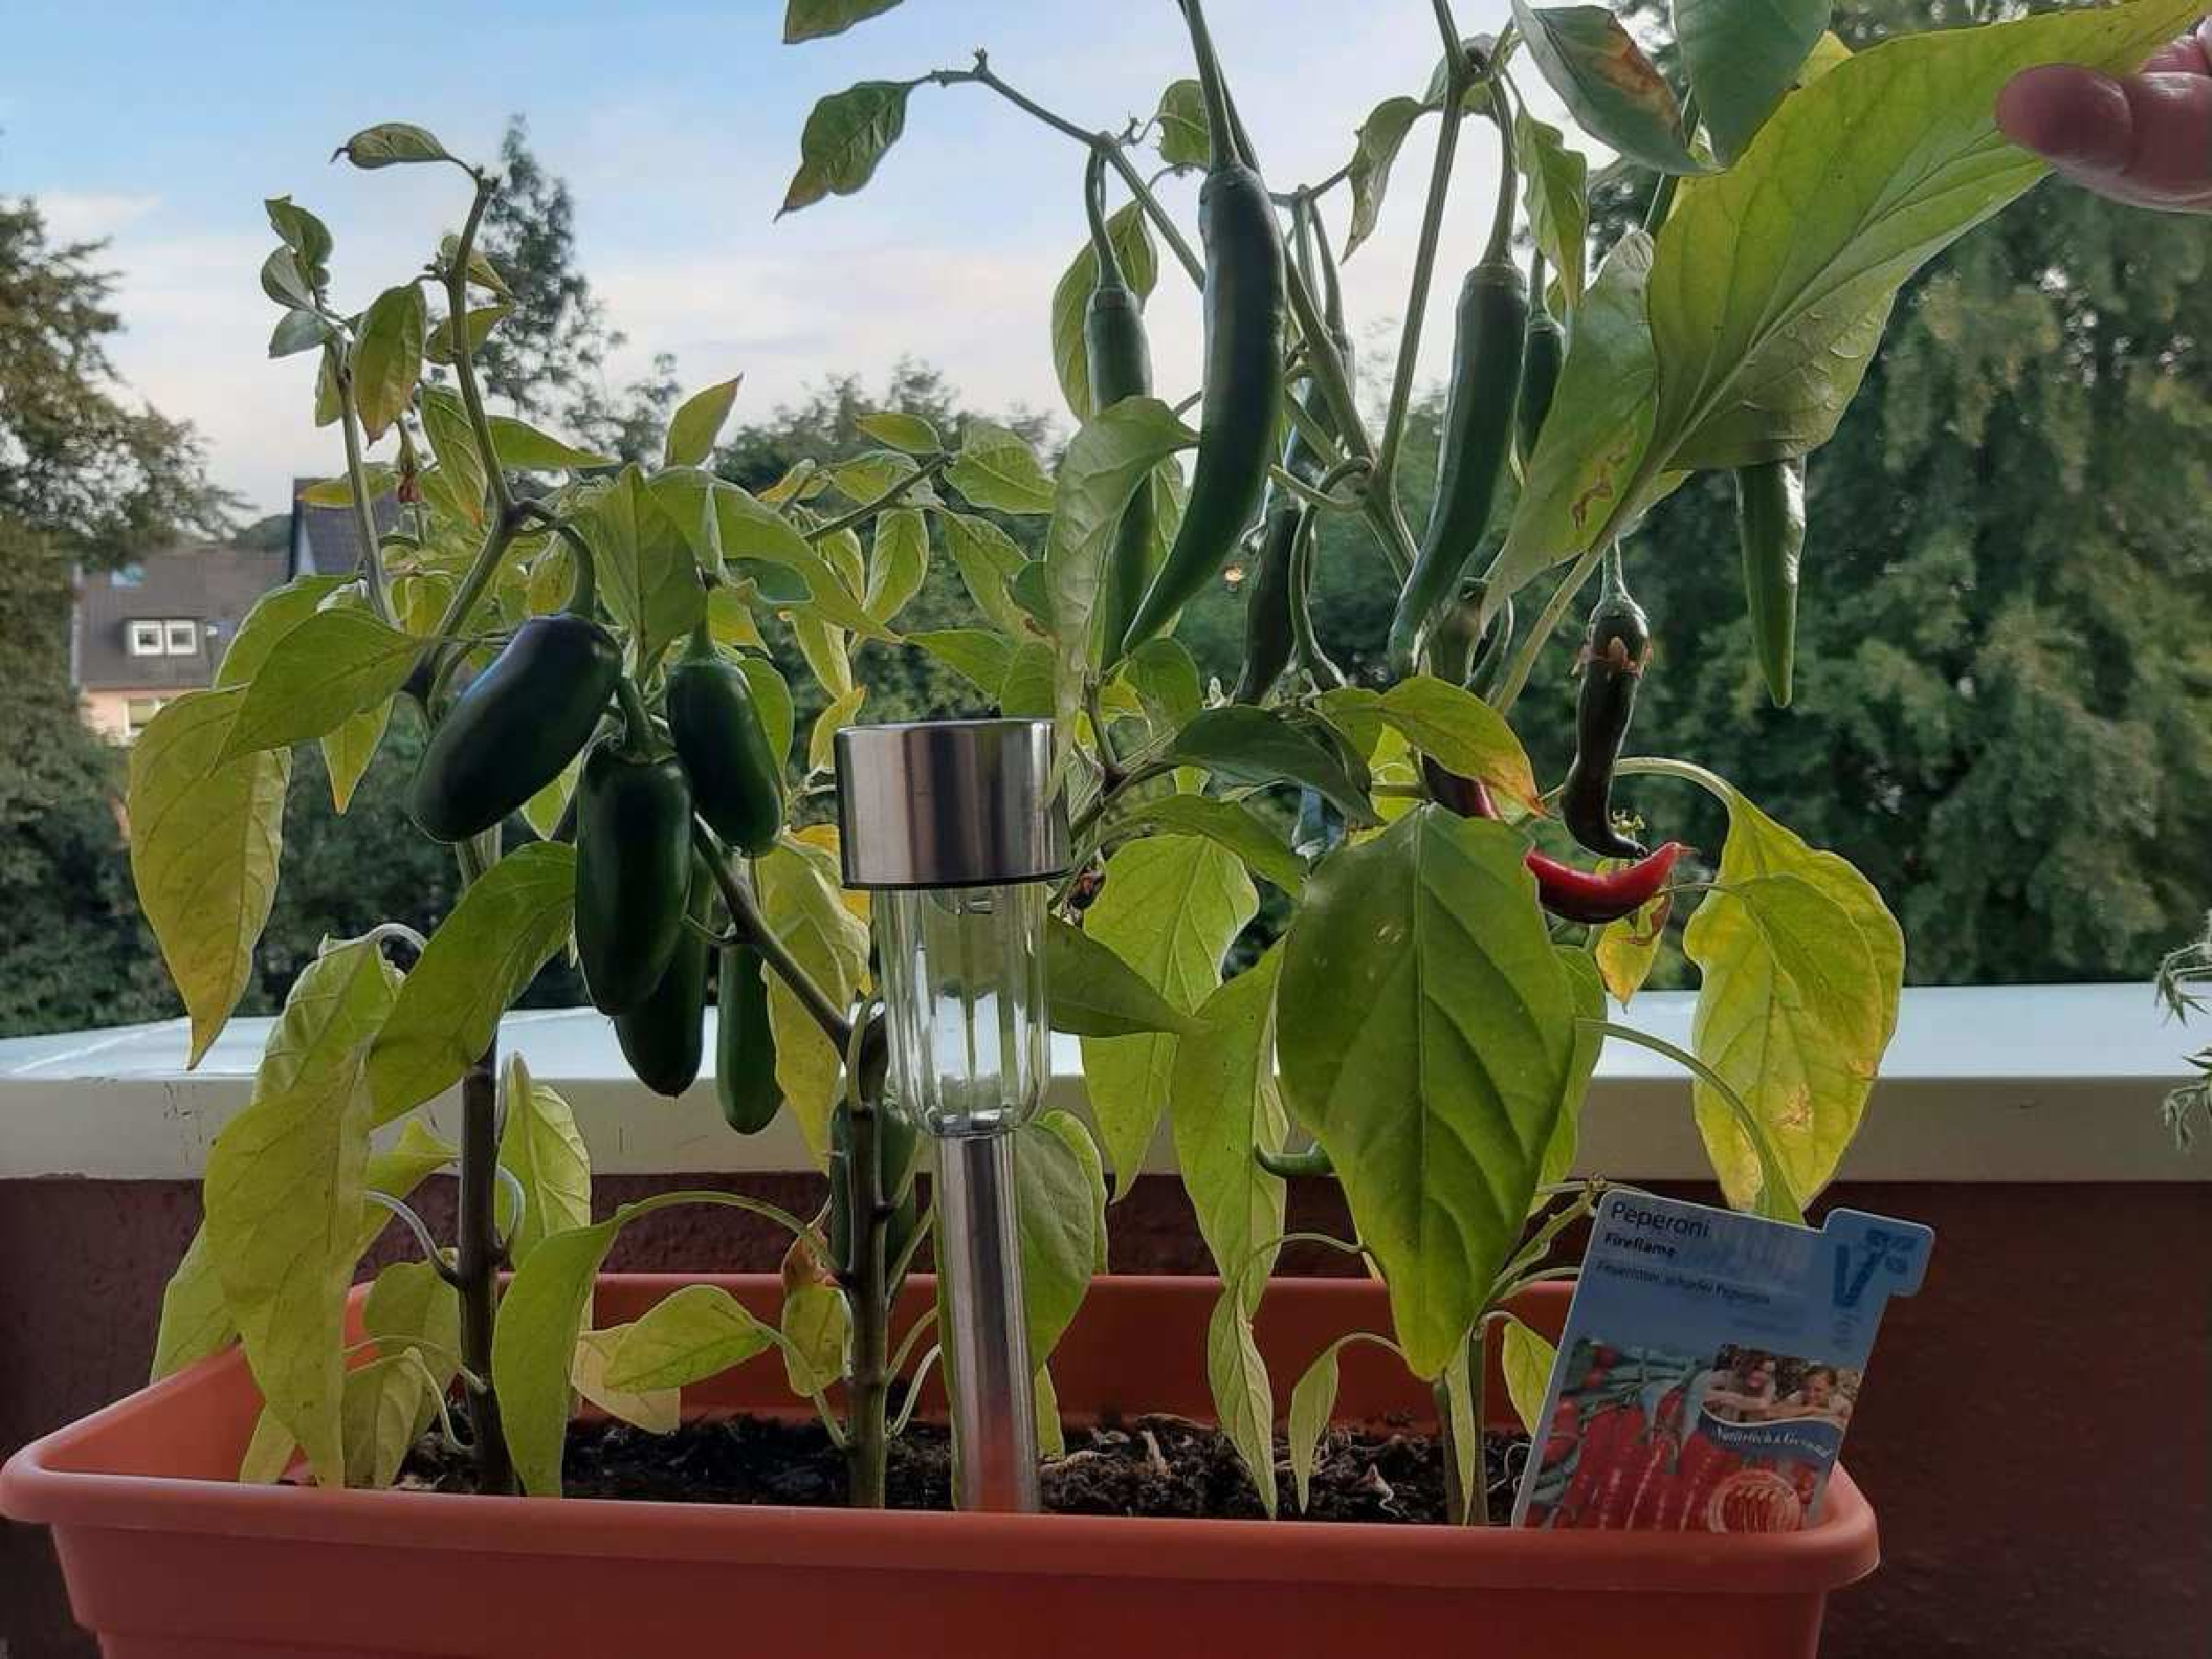
\includegraphics[width=0.6\textwidth]{images/Chili-1.pdf}
\caption{Abbildung-Bsp}
\label{fig:Abbildung-Bsp}%% anpassen
\end{figure}

\lstset{language=TeX}% C, TeX, Bash, Python 
\begin{lstlisting}[
	%caption={}, label={code:}%% anpassen
]
![Abbildung-Bsp](images/Chili-1.pdf){width=60%}
\end{lstlisting}

\section{Tabelle}\label{tabelle}

Tabelle-Bsp vgl.~(\autoref{tab:Tabelle-Bsp}).

\begin{table}[!ht]% hier: !ht 
\centering 
	\caption{Tabelle-Bsp} \label{tab:Tabelle-Bsp}%% anpassen 
\begin{tabular}{@{}rll@{}}
\hline
\textbf{Nr.} & \textbf{Begriffe} & \textbf{Erklärung} \\ 
\hline
1 & a1 & a2 \\ 
2 & b1 & b2 \\ 
3 & c1 & c2 \\ 
4 & a1 & a2 \\ 
\hline
\end{tabular} 
\end{table}

\lstset{language=TeX}% C, TeX, Bash, Python 
\begin{lstlisting}[
	%caption={}, label={code:}%% anpassen
]
| **Nr.** | **Begriffe** | **Erklärung** |
| ------: | :----------- | :------------ |
|       1 | a1           | a2            |
|       2 | b1           | b2            |
|       3 | c1           | c2            |
|       4 | a1           | a2            |
\end{lstlisting}

\section{Mathematik}\label{mathematik}

$[V] = [\Omega] \cdot [A]$ o. $U = R \cdot I$ o. $R = \frac{U}{I}$

\lstset{language=TeX}% C, TeX, Bash, Python 
\begin{lstlisting}[
	%caption={}, label={code:}%% anpassen
]
$[ V ] = [ \Omega ] \cdot [ A ]$ o. $U = R \cdot I$ o. $R = \frac{U}{I}$
\end{lstlisting}

$5~cm$, $a \cdot b$, $\cdots$, $\Omega$

$100^\circ\text{C}$

$80~\%$

\lstset{language=TeX}% C, TeX, Bash, Python 
\begin{lstlisting}[
	%caption={}, label={code:}%% anpassen
]
$5~cm$, $a \cdot b$, $\cdots$, $\Omega$
$100^\circ\text{C}$  
// ACHTUNG: Prozentzeichen macht Probleme in HTML und Latex 
// Z.B. 80 %
$80~\%$ // in Latex
$80~%$  // in HTML
\end{lstlisting}

\textbf{Mathematik-Umgebung}

\begin{equation}
  \sum_{i=1}^5 a_i = a_1 + a_2 + a_3 + a_4 + a_5
\end{equation}

\begin{align*}
    \sum_{i=1}^5 a_i = a_1 + a_2 + a_3 + a_4 + a_5
\end{align*}

\lstset{language=TeX}% C, TeX, Bash, Python 
\begin{lstlisting}[
	%caption={}, label={code:}%% anpassen
]
\begin{align*}
    \sum_{i=1}^5 a_i = a_1 + a_2 + a_3 + a_4 + a_5
\end{align*}
\end{lstlisting}

\section{Texthervorhebung}\label{texthervorhebung}

\textbf{Fett} oder \emph{Kursiv}

\lstset{language=TeX}% C, TeX, Bash, Python 
\begin{lstlisting}[
	%caption={}, label={code:}%% anpassen
]
**Fett** oder *Kursiv*
\end{lstlisting}

\section{Code}\label{code}

Hallo Welt vgl.~(\autoref{code:HalloWelt}).

\lstset{language=C}% C, TeX, Bash, Python 
\begin{lstlisting}[
	caption={Hallo Welt}, label={code:HalloWelt}%% anpassen
]
// hallowelt.c
#include <stdio.h>
int main(void) {
    printf("Hallo Welt!\n");
    return 0;
}
\end{lstlisting}

\section{Links}\label{links}

\url{https://google.de} oder \href{https://google.de}{Google}

\lstset{language=TeX}% C, TeX, Bash, Python 
\begin{lstlisting}[
	%caption={}, label={code:}%% anpassen
]
<https://google.de> oder [Google](https://google.de)
\end{lstlisting}

Fußnote\footnote{\url{https://bw-ju.de/}}

\lstset{language=TeX}% C, TeX, Bash, Python 
\begin{lstlisting}[
	%caption={}, label={code:}%% anpassen
]
Fußnote[^1]       

[^1]: <https://bw-ju.de/>
\end{lstlisting}

\section{Absätze}\label{absaetze}

Dies hier ist ein Blindtext zum Testen von Textausgaben. Wer diesen Text
liest, ist selbst schuld. Der Text gibt lediglich den Grauwert der
Schrift an. Ist das wirklich so? Ist es gleichgültig, ob ich schreibe:
>>Dies ist ein Blindtext<< oder >>Huardest gefburn<<? Kjift -
mitnichten! Ein Blindtext bietet mir wichtige Informationen. An ihm
messe ich die Lesbarkeit einer Schrift, ihre Anmutung, wie harmonisch
die Figuren zueinander stehen und prüfe, wie breit oder schmal sie
läuft. Ein Blindtext sollte möglichst viele verschiedene Buchstaben
enthalten und in der Originalsprache gesetzt sein. Er muss keinen Sinn
ergeben, sollte aber lesbar sein.

Fremdsprachige Texte wie >>Lorem ipsum<< dienen nicht dem eigentlichen
Zweck, da sie eine falsche Anmutung vermitteln.

%\chapter{Sprachlich-formale-Aspekte}
%%\chapter{Sprachlich-formale Aspekte}

Wissenschaftliche Ausarbeitungen dienen der Wissensvermittlung -- es ist überaus wichtig, Lesenden die Informationsaufnahme möglichst einfach zu machen, Inhalte logisch zu gliedern und in guter sprachlicher Form darzustellen.


\section{Textverständlichkeit}

Der Text ist logisch aufzubauen und so zu formulieren, dass er auch für den nicht an der Durchführung der Arbeit beteiligten Lesenden verständlich und nachvollziehbar ist. Die behandelten Themen müssen leicht erkennbar sein. Größere Abschnitte sollten einen kurzen Überblick über ihre Inhalte geben. Die Verständlichkeit des Textes kann durch die Verwendung von kurzen Sätzen, einer einfachen, aber fachsprachlich korrekten Wortwahl und durch die Vermeidung von Füllworten und überflüssigen Fremdworten wesentlich erhöht werden.

\begin{itemize}
\item Keine Prosa, sondern präzise Begriffe und Sätze!
\item Eine einheitliche Terminologie verwenden, damit Begriffe wiedererkannt werden können.
\item Zentrale Begriffe klären und die Arbeit für interessierte Laien verständlich halten.
\item Pure Textblöcke, die sich über mehrere Seiten erstrecken, sind ein Zeichen für mangelnde strukturelle Leseunterstützung. Weiter unterteilen oder variantenreichere Inhaltsarten (Schriftarten, Listen, Diagramme, Tabellen, \ldots) einsetzen.
\item Das schnelle überfliegen des Textes und das Springen in der Arbeit muss aktiv unterstützt werden. Lesende müssen jederzeit die wesentlichen gerade diskutierten Themen schnell erkennen und auch bestimmte vorher schon einmal gelesene Fakten schnell wiederfinden können.
\item Kurz einen Gesamtüberblick (Einordnung ins >>große Bild<<, eine Tabelle) geben und dann tiefer in die Details. Z. B. vor dem Start einer Reihe von Subsections die verschiedene Ausprägungen eines Sachverhalts diskutieren, diese Sachverhalte vorher alle aufzählen und kurz erläutern.
\item Fremdworte/Fachbegriffe nicht einfach ohne weitere Erläuterung verwenden und als bekannt voraussetzen. Selbst wenn der Begriff etabliert und bekannt scheint -- das ist oft auch nur in einem Teilgebiet (der Informatik) so. Deshalb generell Fachbegriffe und Fremdworte erläutern.
\item Die einzelnen Abschnitte sollten entsprechend auf einander verweisen. Überleitungen und Zusammenfassungen zwischen Kapiteln sind hilfreich.
\item Zu Beginn eines Kapitels ist eine Übersicht über dessen Inhalt sinnvoll. Am Ende eines Kapitels kann eine Überleitung zum nächsten Kapitel helfen, den roten Faden aufzuzeigen.
\item Gute Überschriften, vielseitige Präsentation der Inhalte (Diagramme, Tabellen, Auflistungen, \ldots) und aussagekräftige Inhaltsunterschriften verwenden.
\item Durch eine Kombination aus Text und Bild lassen sich komplexe Sachverhalte vereinfacht darstellen und verständlich vermitteln.
\item Verwendet sprechende Titel für Kapitel/Sections/\ldots! Nicht einfach nur >>Aufbau<<, >>Mechanismen<<, >>Dritter Schritt<<, etc. Man sollte nicht erst den Text lesen müssen, um den Kontext zu verstehen. Viel besser: >>Aufbau einer Ausführungsumgebung für Microservices<<, >>Mechanismen zur Fehlervermeidung und Fehlerbeseitigung<<, >>Dritter Schritt: Implementierung der Schnittstellen zwischen Diensten<<.
\item Statt in der Textform z. B. >>mittels einerseits \ldots andererseits<<,\\>>erstens\ldots zweitens\ldots drittens<< o. ä. lieber Aufzählungszeichen verwenden. Dies unterstützt die Lesbarkeit teilweise enorm.
\item Möglichkeiten zur Hervorhebung (z. B. Fettdruck) und Textstrukturierung (Gedankenstriche, Klammern, Semikolon, Doppelpunkt, \ldots) nutzen.
\end{itemize}



\section{Ausdruck \& Stil}

Eine wissenschaftliche Ausdrucksweise ist sachlich, präzise und bemüht sich um Objektivität. Die Verwendung umgangssprachlicher Ausdrücke, schwammiger Formulierungen und übertriebener literarischer Stilmittel (z. B. Verwendung von Synonymen) stören die wissenschaftliche Ausdrucksweise.

\begin{itemize}
\item Umgangssprachliche Formulierungen vermeiden (>>von vorneherein<<, >>wird es richtig teuer<<, >>ziemlich simpel<<, >>Gehen wir das ganze einmal durch<<, >>zum Laufen zu bringen<<, >>sprich\ldots<<, >>Fazit: \ldots<<, >>Ich habe mir gedacht,\ldots<<)
\item Komponenten nicht personifizieren (>>der JBoss/er<<, >>die Apaches<<, >>JBosse<<).
\item    Vermeidet das Wort >>offensichtlich<<. Das wirkt, als hieltet ihr die Lesenden für dumm.
\item    Vermeidet Füllwörter wie >>sehr<<. Wenn etwas >>sehr wichtig<< ist, dann sind in der Schriftsprache Worte wie >>zentral<<, >>fundamental<<, >>essentiell<<, etc. eleganter.
\item    Worte wie >>sehr<<, >>relativ<<, >>ziemlich<<, >>quasi<<, >>gewissermaßen<< sind in den allermeisten Fällen überflüssig und ungenau.
\item    Die Begriffe, für die Demonstrativpronomen (dieser/jener/welcher) Stellvertreter sind, müssen eindeutig erkennbar sein.
\item    Nicht zu umständliche Stellvertreterausdrücke verwenden (>>der zur Diskussion stehende Sachverhalt<<, >>die vorbezeichneten Gegenstände<<, etc.) -- da müssen Lesende viel zu viel nachdenken (und erstmal den Lesefluss stoppen und nachgucken, welche drei Sachen eigentlich gemeint sind).
\item    Nicht verschiedenste Synonyme für ein und denselben Begriff verwenden -- insbesondere, wenn der Begriff etabliert ist (Negativbeispiel: >>künstliche neuronale Netze<<, >>artifizielle Netze<<, >>die in Rede stehenden Netze<<, >>ebenjene Netze<<, >>die beschriebenen Netze<<)
\end{itemize}



\section{Rechtschreibung \& Grammatik}

Mindestens ebenso wichtig wie die Verständlichkeit ist die sprachliche Korrektheit. Ausarbeitungen müssen hinsichtlich Rechtschreibung, Grammatik, Satzbau und Zeichensetzung ohne Fehler sein. Ein nennenswerter Fehleranteil wird oft als Indikator für mangelnde Sorgfalt und Ernsthaftigkeit der Arbeit gewertet. Solche Arbeiten werden nicht anerkannt auch nicht als Vor-Version!).

\begin{itemize}
\item Alles, was die Rechtschreibkontrolle nicht kennt, ist entweder falsch geschrieben oder muss als Fremdwort, Eigenname, \verb|\code| etc. hervorgehoben sein.
\item Es empfiehlt sich generell, Freunde, Kommilitonen, und eine Software zur Prüfung der Rechtschreibung \& Grammatik nochmal auf den Text schauen zu lassen. Als Autor bekommt man schnell einen Tunnelblick und sieht die Fehler nicht mehr.
\item Beachtet schwierige Wörter. >>zum einen<<, >>zum anderen<<, >>des Weiteren<<
\item Regeln für das Setzen von Bindestrichen: Deutsch > immer (>>Hasso-Plattner-Institut<<), Englisch > in der Regel nicht (>>Hasso Plattner Institute<<), Deutsch+Englisch > kombiniert (>>Java EE-Sicherheitsmodell<<). Im Deutschen kommt es äußerst selten vor, dass Worte weder Bindestrich haben noch zusammengeschrieben werden können. Es heißt z. B. nicht >>Download Modus<<, sondern >>Download-Modus<< oder (da Download im Duden steht) >>Downloadmodus<<.
\item Zu einem >>einerseits<< muss es ein >>andererseits<< geben, zu einem >>erstens<< auch ein >>zweitens<<, zu einem >>sowohl<< auch ein >>als auch<<, usw.
\end{itemize}

Schreibung von Zahlen (deutsch):

\begin{itemize}
\item Zahlen von eins bis zwölf werden in der Regel ausgeschrieben. Ansonsten nur ein- und zweisilbige Zahlwörter (hundert, tausend, \ldots)
\item Vor Zeichen, Abkürzungen von Maßen, Gewichten, Geldsorten usw. ist die Zahl in Ziffern zu schreiben: 3 km; 7,4 kg; 6 EUR. Steht statt der Abkürzung die entsprechende Vollform, kann man sowohl in Ziffern als auch in Buchstaben schreiben: 11 Kilometer/elf Kilometer; 2 Euro/zwei Euro.
\item Die Zahlen von 13 an können -- sofern sie Übersichtlich sind -- auch ausgeschrieben werden.
\item Im IT-Bereich gibt es sehr oft einen Unterschied zwischen 0 (dem Zahlenwert) und null (dem Nullwert/NIL, Fehlen eines Wertes)!
\item Zahlen sollten zur besseren Lesbarkeit in Dreiergruppen gegliedert werden, und zwar sowohl links als auch rechts des Dezimaltrennzeichens. Laut ISO 80000 soll das Tausendertrennzeichen ein schmales Leerzeichen sein, niemals ein Komma, Punkt oder irgendein anderes Zeichen. Zahlen sollten (außer bei tabellarischer Darstellung) erst ab fünf Stellen untergliedert werden.
\item Sätze nie mit Konjunktionen (>>und<<, >>oder<<, >>aber<<, sondern) beginnen. Konjunktionen sind -- wie der Name schon sagt -- Verbindungswörter und stellen die syntaktische Verbindung zwischen Wörtern, Satzteilen oder Sätzen her.
\end{itemize}


\section{Grafiken, Tabellen \& Codeausschnitte}

Jede Fließumgebung (Grafiken, Graphen, Diagramme, Tabellen, Codeausschnitte, \ldots) muss beschriftet sein (>>captions<<).

\begin{itemize}
\item Die Beschreibungen der Abbildungen, Tabellen, Diagramme, Quellcode, etc. müssen jene auch ohne Kontext beschreiben -- erläutern, was man alles sehen und erkennen kann. So muss man beim Betrachten nicht zurück in den Fließtext springen.
\item In jeder Beschriftung müssen folgende Fragen beantwortet werden: Was ist dargestellt? Welche Besonderheiten sind zu erkennen? Welche Rückschlüsse ergeben sich daraus für den momentan behandelten Sachverhalt?
\item Die Achsen von Diagrammen ordentlich beschriften (Metrik und Einheiten). Bei Vergleichen angeben, ob große oder ob kleine Werte besser sind. Fehlerbalken verwenden.
\item Wenn Text in den Abbildungen auf Englisch ist, man aber einen deutschen Text schreibt: Entweder den Text in der Abbildungen übersetzen, oder die Bildunterschrift so gestalten, dass man das auch verstehen kann, wenn man kein Englisch kann.
\item Bilder so skalieren, dass die Textgrößen verschiedener Abbildungen etwa konsistent sind und nicht sehr viel größer (oder kleiner) als die normale Textschriftgröße.
\item Grafiken, Tabellen etc. müssen auch im Text referenziert werden um die Verbindung zwischen Text und Abbildungen herzustellen.
\end{itemize}

\section{weitere wichtige Formalien}

Bei den Formalien gibt es verschiedene Möglichkeiten -- die Grundregel sollte jedoch sein: Hauptsache einheitlich, Übersichtlich und systematisch!

\begin{itemize}
\item Fachbegriffe, Produkt-/Eigennamen und fremdsprachlichen Begriffen (z. B. Java EE, Java Virtual Machine, Enterprise Services, Application Client Container) bei der ersten Verwendung kenntlich machen (z. B. mittels \verb|\emph|) und auch eine kurze Erläuterung mit hinzufügen. Oft lässt sich das Erläutern eines Fremdworts/Fachbegriffs leicht durch eine Übersetzung implementieren; manchmal aber auch nicht: Dann muss ein Nebensatz, eine Fußnote o. ä. investiert werden, um den Fachbegriff/das Fremdwort genauer zu erklären. Danach kann auch das Fremdwort normal verwendet werden.
\item Bei englischen Begriffen, die leicht durch deutsche Begriffe ersetzt werden können, dies bitte auch tun (z. B. >>Interface<< vs. >>Schnittstelle<<, >>Button<< vs. >>Schaltfläche<<).
\item Abkürzungen sind grundsätzlich bei ihrer ersten Verwendung einmal aufzuschlüsseln. Auch Begriffe, die im Glossar erwähnt sind, sind bei der ersten Verwendung in der Arbeit noch einmal kurz zu erläutern (z. B. Pan- und Pitch-Gesten).
\item Bei Verwendung von Unterpunkten müssen mindestens zwei Unterpunkte vorhanden sein (also >>2.<< >>2.1<< >>2.2<< \ldots >>3.<< statt >>2<< >>2.1<< >>3<<).
\item Eine Section, auf die sofort eine Subsection (ohne Text dazwischen) folgt, ist unschön.
\item Bei Nennung von Produkten die URL der Bezugsquelle als Fußnote angeben.
\item URLs nicht in den Fließtext integrieren, sondern als Fußnote oder ggf. als Referenz darauf verweisen (sonst unterbrechen sie durch ihre Länge den Lesefluss). Bei Verwendung von LaTeX die URLs immer auch in die \verb|\url|-Umgebung einfügen.
\item Schreiben in der ersten Person Singular vermeiden. >>Ich<< ist üblicherweise nur akzeptabel, wenn es um eigene Leistungen/Beiträge geht.
\item Aufzählung einzelner Begriffe nur machen, wenn sie in der Auflistung noch etwas genauer erklärt werden. Ansonsten einfach als Fließtext hintereinander aufschreiben.
\item Sind Subsections wirklich immer nötig? Oder tut es vielleicht auch eine einfache Auflistung?
\item Keine zusätzlichen Formatierungen in Überschriften verwenden.
\end{itemize}



\section{spezielle Hinweise für Ausarbeitungen, die mit LaTeX bearbeitet werden}

\begin{itemize}
\item Absätze nicht mit \verb|\\| trennen, sondern durch eine Leerzeile. Die beiden Sachen sehen im erstellten Dokument unterschiedlich aus (sonst werden z. B. die Absätze nicht eingerückt).
\item Für Gedankenstriche bitte \verb|--| benutzen (doppeltes Minus).
    Mithilfe einer \verb|~| (Tilde) kann ein geschütztes Leerzeichen (engl. no-break space) eingefügt werden, dass einen automatischen Zeilenumbruch an dieser Position verhindert (bzw. verzögert) und dadurch die Lesbarkeit verbessert (z. B. \verb|123~kg|, \verb|3~Liter|, \verb|DB~Systel|, \verb|S.~42~ff.| oder auch zur Umbruchsteuerung bei Titel-Angaben).
\item Bei allen Quellen, die im Quellenverzeichnis auftauchen sollen, muss irgendwo eine Referenz darauf existieren (kein \verb|\NoCite|!).
\item URLs bitte in die \verb|\url|-Umgebung einfügen, möglichst in eine Fußnote (\verb|\footnote|) packen, den Seitentitel nennen und ggf. das Abrufdatum angeben.
\item Kein \verb|\emph| o. ä. in Überschriften verwenden.
\item Literaturverzeichnis: Als *.bib-Datei!
\item Bei Firmen-/Organisationsbezeichnungen im author-Feld die sich aus mehreren Wörtern zusammensetzen (und die keine Vornamen/Nachnamen sind) diese separat in \verb|{}| packen. Zum Beispiel \verb|{{Microsoft Corporation}}| (damit sie nicht als Vor-/Nachname formatiert werden).
\item Bei mehreren Autoren diese nicht mit Komma voneinander trennen, sondern mit and.
\end{itemize}



\section{Korrektur \& Abgabe}

Eine gute schriftliche Ausarbeitung braucht eine gute Argumentation und eine gute Schlussüberarbeitung. Diese sind jedoch nicht nach ersten Niederschrift fertig -- daher sind mehrere Überarbeitungen vor Abgabe der Endfassung unbedingt notwendig. Kurze und präzise Formulierungen entwickelt man nicht beim ersten Nachdenken über ein Problem. Logikfehler oder fehlende Argumente fallen nicht sofort auf.

\begin{itemize}
\item Den Text mehrfach lesen und überarbeiten.
\item Wiederholungen beseitigen, Abschnitte eventuell umstellen, umformulieren, Brüche glätten, Teile verbinden, Aussagen präzisieren, an der Sprache feilen.
\item Den roten Faden durchgängig kenntlich machen, die Fragestellung und Argumentation schärfen, deren Nachvollziehbarkeit überprüfen.
\item Möglichst auch noch einmal eine (externe) Rechtschreibkontrolle zu Rate ziehen -- eine korrekte Rechtschreibung und Grammatik sind ein Muss!
\item Ebenfalls solltet ihr vor der Abgabe eines Dokuments noch einmal (gründlich) nachschauen, ob alles so aussieht, wie es soll passt das Layout, wurden alle (gravierenden) overfull-Boxes beseitigt, sind die Referenzen ordentlich gesetzt, ist das Literaturverzeichnis vorhanden usw.
\item Wichtig ist auch, dass ihr euch jeden einzelnen Eintrag im Literaturverzeichnis noch einmal anschaut -- sind notwendigen Angaben alle dargestellt, ist die Autorenliste korrekt, sieht man bei Online-Quellen auch die Adresse etc.
\end{itemize}

\section{Drucken \& Binden}

Nach dem Schreiben der Abschluss-Arbeit muss diese noch gedruckt und gebunden werden. Damit das möglichst hochwertig, schnell und preiswert geschehen kann, solltet ihr folgende Dinge beachten:

\begin{itemize}
\item \emph{Papierstärke} Für den Ausdruck bitte ordentliches Papier verwenden (so, dass man die Rückseite nicht durchschimmern sieht). Um professionell zu wirken, sollte Papier mit mind. $100~g/m^2$ gewählt werden.
\item \emph{Bindung} Wir raten dazu, beim Binden ein >>Softcover mit Aufdruck auf der Vorderseite<< zu wählen; ein Hardcover geht natürlich auch, ist allerdings etwas teurer. Beide Bindungsmöglichkeiten haben ein professionelles Aussehen und sind sehr langlebig. Falls zum Binden ein Plastikbinderücken verwendet werden sollte -- bitte auch einen Binderücken wählen, der zur Papierstärke passt. Das sieht sonst lächerlich aus. Die Plastikbindung ist eine günstige Lösung; im Gegensatz zu anderen Bindungsmöglichkeiten wirkt es allerdings weniger professionell. Denkt schon vor dem Drucken ggf. an eine Bindungskorrektur (diese kann in der Vorlage \emph{praeambel.sty} mittels \verb|\bcor| eingestellt werden).
\end{itemize}

%\chapter{Text-Formatierungen}
%%\chapter{Beispiel für Formatierungen}

Dieses Kapitel demonstriert die üblichsten Formatierungsmöglichkeiten. Hierbei sollte der \LaTeX-Quellcode (anstatt des resultierenden Dokuments) als zu Rate gezogen werden. :-)


\verb|\textbf| \textbf{Ein formatierter Text} normaler Text \verb|\emph|  \emph{Ein formatierter Text} normaler Text \verb|\footnote| \footnote{Fussnote}. \verb|\enquote| \enquote{Anführungszeichen} oder >>Anführungszeichen<<

12~Byte, 6~kg, 100~EUR, 1--12, 299~792~458~m/s, 3~Liter, von \ldots bis \ldots

$12~Byte, 6~kg, 100~EUR, 299~792~458~m/s, 3~Liter$

\verb|12~Byte|, \verb|6~kg|, \verb|100~EUR|, \verb|1--12|, \verb|299~792~458~m/s|, \verb|3~Liter|, \verb|von \ldots bis \ldots|

Liste der recht­schreib­lich schwieri­gen Wörter\footnote{\url{https://www.duden.de/Liste-der-rechtschreiblich-schwierigen-Woerter}}.

Rechtschreibkontrolle - eine korrekte Rechtschreibung und Grammatik sind ein Muss!\footnote{\url{https://languagetool.org/de/}}.



\section{Aufzählungen}

\begin{itemize}
	\item a
	\item b
\end{itemize}

\begin{enumerate}
	\item eins 
	\item zwei
\end{enumerate}


\begin{description}
	\item[Beschreibung...] xyz 
	\item[Beschreibung...] zyx
\end{description}


\section{Gliederung -- Abschnitte, Unterabschnitte \& Absätze} \label{sec:structure}
Ein (Latex-)Dokument lässt je nach Dokumentenklasse (nicht jede Klasse unterstützt jede Untergliederung) unterteilen bzw. gliedern. In diesem Dokument stehen folgende Befehle zur Verfügung:
\begin{itemize}
	\item \verb|\chapter{...}|
	\item \verb|\section{...}      \label{sec:...}|
	\item \verb|\subsection{...}   \label{subsec:...}|
	\item \verb|\subsubsection{...}\label{subsubsec:...}|
	\item \verb|\paragraph{...}    \label{par:...}|
	\item \verb|\subparagraph{...} \label{subpar:...}|
\end{itemize}

\section{Referenzen}

\paragraph{Verweise (label + autoref)}
\verb|\autoref| \& \verb|\label| Text (\autoref{code:one}). Text (\autoref{fig:Chicken1}) Text \autoref{tab:tabneu} Text \autoref{sec:structure}.

\paragraph{Quellenangaben (cite)}
\verb|\cite| Text\cite{monk:2014:raspberry} Quelle: ~\cite{kofler:2015:raspberry}

\paragraph{Quellenangaben (textcite)}
\verb|\textcite| Text \textcite{monk:2014:raspberry} Quelle: ~\textcite{kofler:2015:raspberry}

\paragraph{Quellenangaben (footfullcite)}
\verb|\footfullcite| Text\footfullcite{monk:2014:raspberry} Quelle: ~\footfullcite{kofler:2015:raspberry}

\emph{Aplpe TV}\footnote{\url{http://www.aplpe.cmo}}


\section{Abbildungen}

Text (\autoref{fig:Chicken1}).
\begin{figure}[!hb]% hier: !hb
	\centering
	\includegraphics[width=0.4\linewidth]{images/logo}
	\caption{Chicken chien}\label{fig:Chicken1}%% anpassen
\end{figure}

Text (\autoref{fig:Chicken2} und \autoref{fig:Chicken1}).

\begin{figure}[!hb]% hier: !hb
	\centering
	\includegraphics[height=0.4\linewidth,angle=90]{images/logo}
	\caption{Bild 90 Grad drehen.}\label{fig:Chicken2}%% anpassen
\end{figure}


\section{Quelltext}
\verb|\lstinline| oder \verb|\verb|.

\paragraph{verb}
Bsp. \verb|int|, \verb|bool| (\autoref{code:one}).

\paragraph{lstlisting}

\lstset{language=C++}% C, TeX, Bash, Python
\begin{lstlisting}[%% anpassen
caption={Es ist eine alte Tradition, eine neue Programmiersprache mit einem Hello-World-Programm einzuweihen. Auch dieses Buch soll mit der Tradition nicht brechen, hier ist das Hello-World-Programm in C++}, label=code:one]
// Ein- und Ausgabebibliothek
#include <iostream>

int main(){// Hauptfunktion
	std::cout << "Hallo Welt!" << std::endl;// Ausgabe
	return 0;
}
\end{lstlisting}

\section{Tabellen neu}

(\autoref{tab:tabneu}).
\begin{table}[!ht]% hier: !ht
	\centering 
	\caption{Tabelle neu, gute Beschreibung einfügen}\label{tab:tabneu}%% anpassen
	\begin{tabular}{@{}rlc@{}}
	\toprule 
    \textbf{Nr.} & \textbf{Begriffe} & \textbf{Erklärung}\\
	\midrule
    1 & a1 & a2\\
    2 & b1 & b2\\
    3 & c1 & c2\\
    4 & a1 & a2\\
	\bottomrule
 	\end{tabular}
\end{table}


\section{Gleichungen}

$x$--$y$, \( x^2 + y^2 = 1 \)

(\autoref{eq:summe}).
\begin{equation}\label{eq:summe}%% anpassen
	\sum \limits_{i=1}^n i = \frac{n(n+1)}{2}
\end{equation}




%\chapter{vorlage-abbildungen}
%\textbf{Vorlage -- Abbildungen}

Abbildung1 (\autoref{fig:Abbildung1}).
%
\begin{figure}[!hb]% hier: !hb
	\centering
	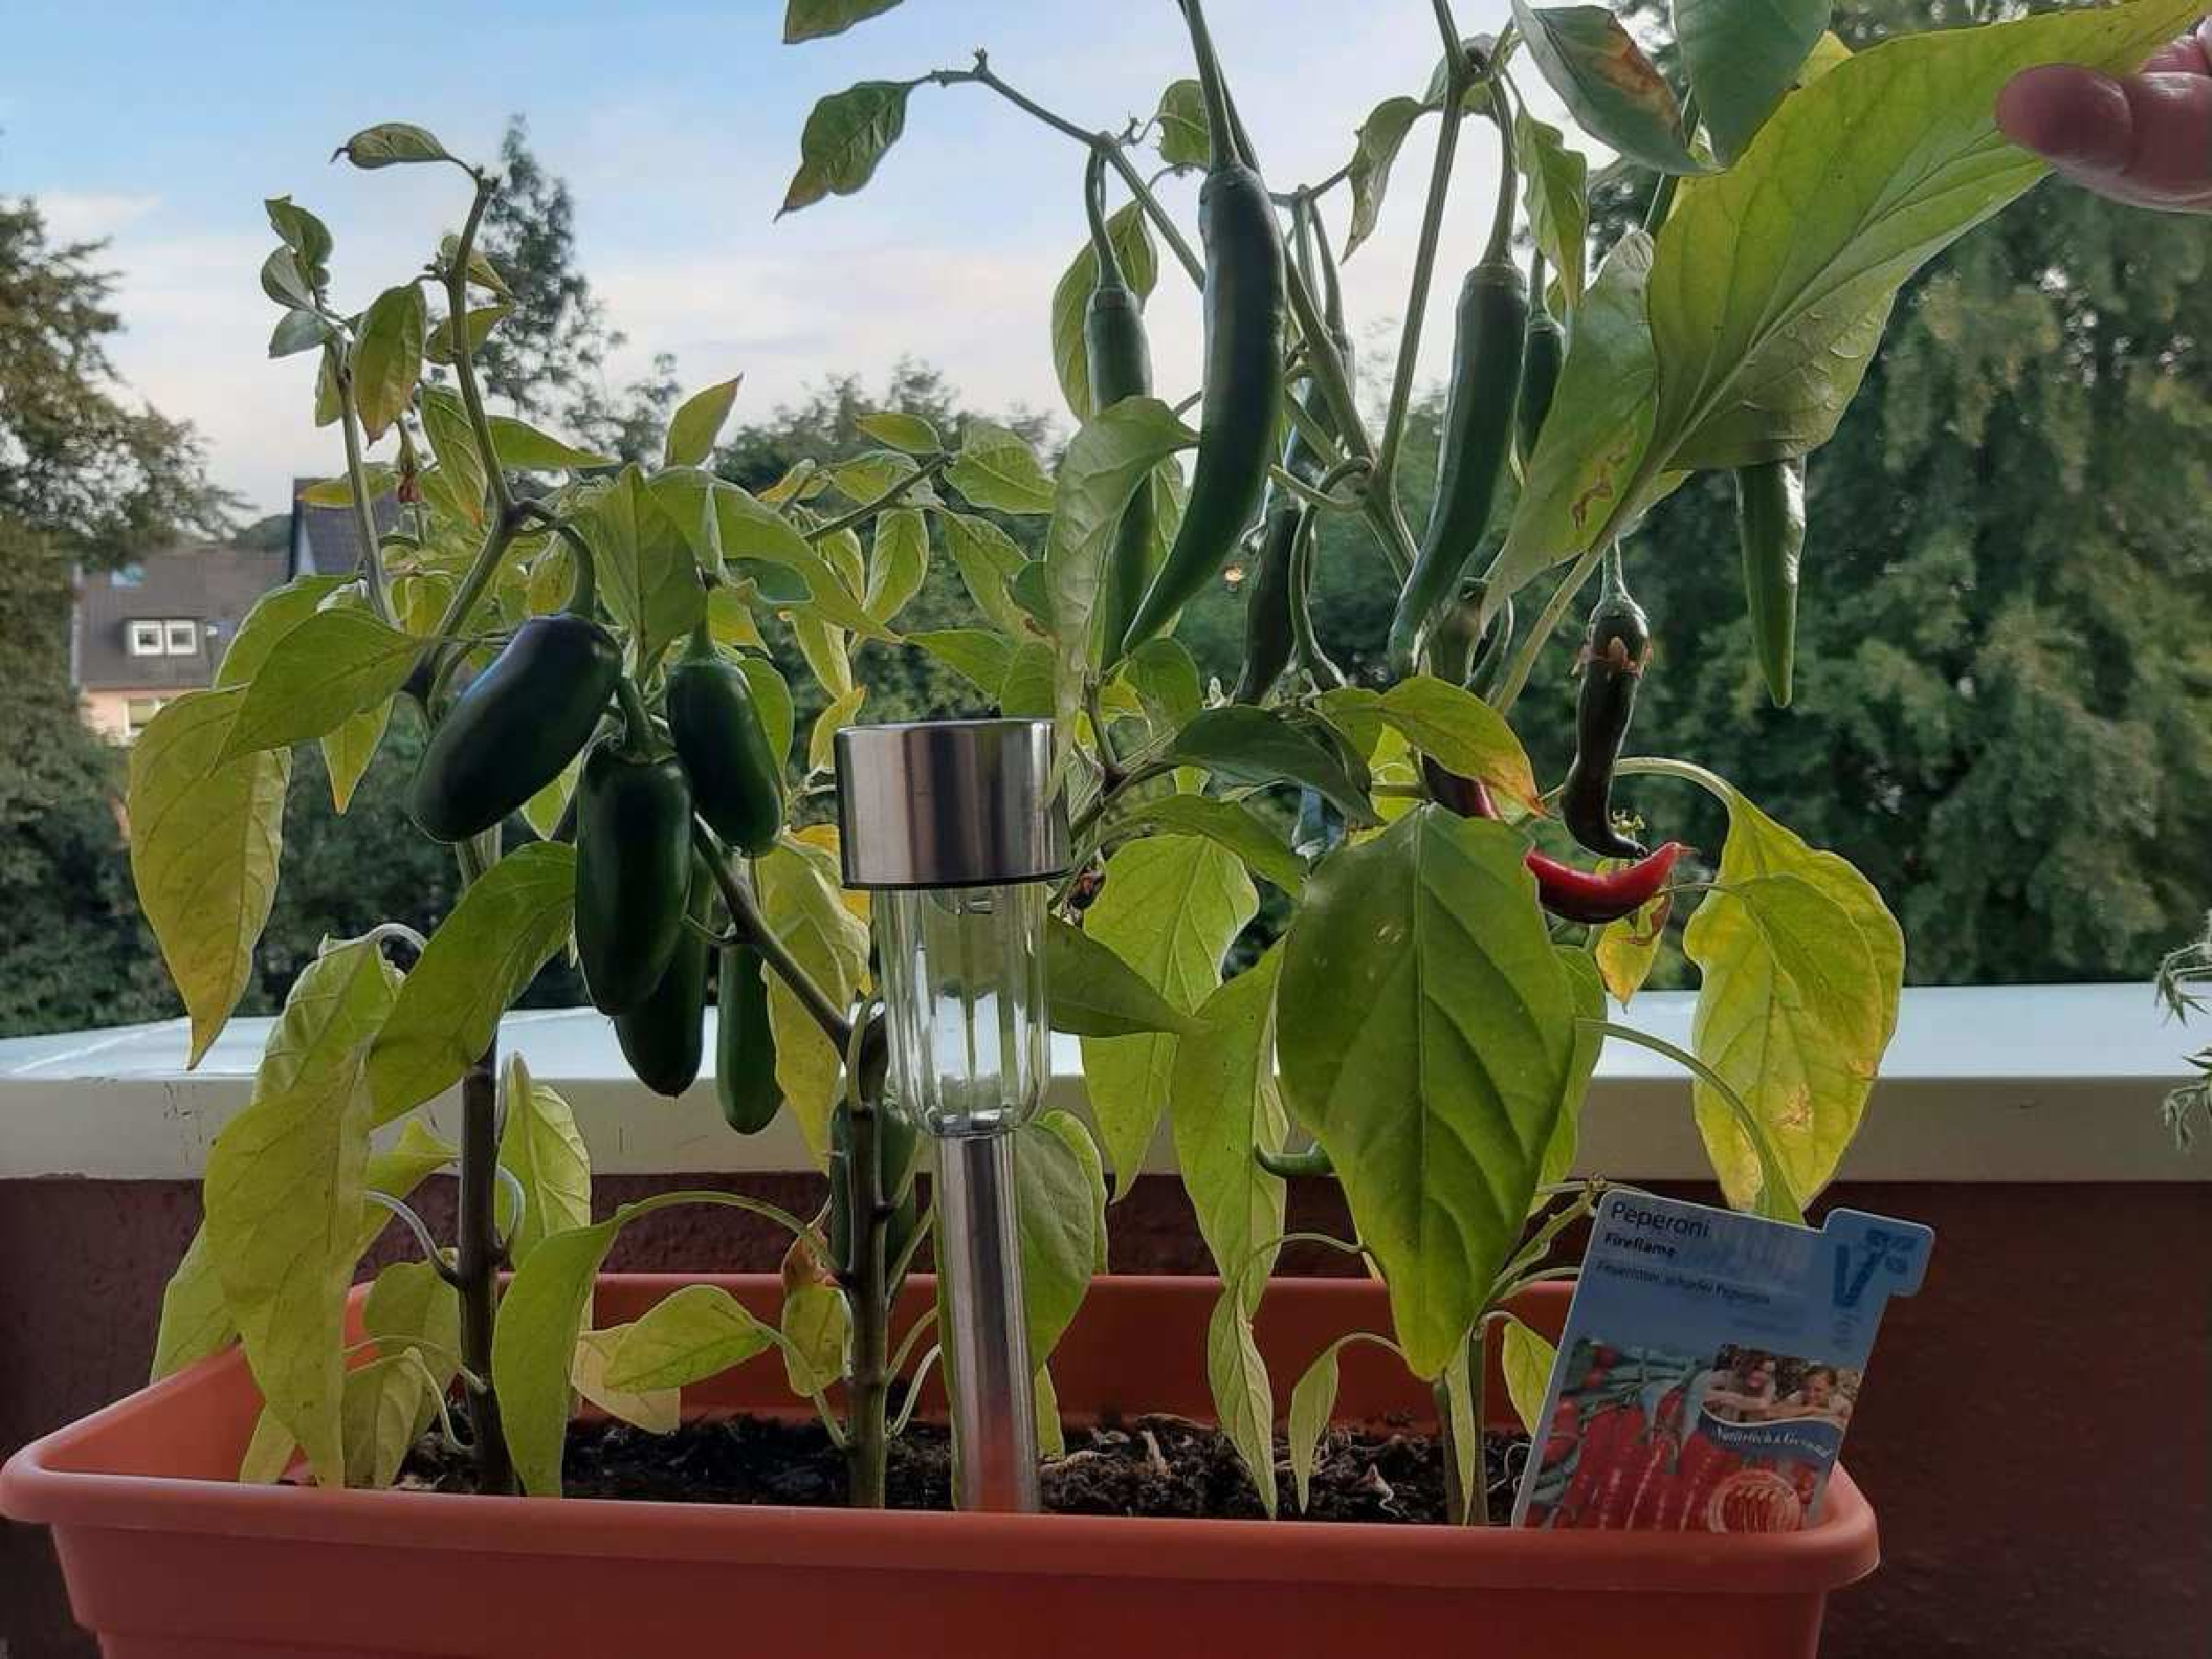
\includegraphics[width=.60\textwidth]{images/Chili-1.pdf}%
	\caption{Abbildung1}\label{fig:Abbildung1}%% anpassen
\end{figure}

Abbildung2 (\autoref{fig:Abbildung2}).
%
\begin{figure}[!hb]% hier: !hb
	\centering
	\includegraphics[width=.95\textwidth]{images/Logo-Details.eps}%
	\caption{Abbildung2}\label{fig:Abbildung2}%% anpassen
\end{figure}


Logo in Neg, Grau, Schwarz (\autoref{fig:logoneggrauschwarz}).
%
\begin{figure}[!hb]% hier: !hb
	\centering
	\begin{minipage}[b]{0.40\textwidth}
		\includegraphics[width=\textwidth]{images/Logo-negativ.eps}%
	\end{minipage}
	\hfill
	\begin{minipage}[b]{0.30\textwidth}
		
\includegraphics[width=\textwidth]{images/Logo-Grau.eps}%
	\end{minipage}
	\hfill
	\begin{minipage}[b]{0.20\textwidth}
		\includegraphics[width=\textwidth]{images/Logo-SW.eps}%
	\end{minipage}
	\caption{Logo in Neg, Grau, Schwarz}\label{fig:logoneggrauschwarz}%% anpassen
\end{figure}



%\chapter{vorlage-literaturangabe-kfz}
%% letztes Update: 28-Jul-20
\textbf{Zitat -- KFZ}

Quelle: ~\textcite{schmidt:2015:klima}

Quelle: ~\textcite{sternbeck:2015:bremsen}

Quelle: ~\textcite{schneehage:2018:aktoren}

Quelle: ~\textcite{frei:2017:hochvolt}

Quelle: ~\textcite{frei:2013:elektrik}

Quelle: ~\textcite{gunther:2019:commonrail}

Quelle: ~\textcite{peter:2015:benzindirekt}

Quelle: ~\textcite{schneehage:2014:sensoren}

Quelle: ~\textcite{frei:2018:vernetztesysteme}

Quelle: ~\textcite{bosch:2020:training}

%\chapter{vorlage-literaturangabe-sport}
%% letztes Update: 28-Jul-20
\textbf{Zitat -- Sport}

\textbf{Kraft}

Quelle: ~\textcite{lauren:2014:fit90tage}

Quelle: ~\textcite{lauren:2016:fitkraftstoff}

Quelle: ~\textcite{lauren:2017:fit}

\textbf{Laufen}

Quelle: ~\textcite{marquardt:2015:laufbibel}

Quelle: ~\textcite{steffny:2006:laufbuch}

Quelle: ~\textcite{zeller:2017:hindernis}

\textbf{Lauftechnik verbessern}

Quelle: ~\textcite{marquardt:2018:laufstil}

\textbf{Fußtraining}

Quelle: ~\textcite{marquardt:2018:fusstraining}

Quelle: ~\textcite{marquardt:2018:fusstrainingsplan}

\textbf{Trainingsrechner}

\begin{itemize}
\item
  Tempo und die Durchgangszeiten Wettkampf
\item
  Schrittfrequenz
\item
  Zeit/Gewicht
\item
  Lauftempo in Min/km, km/h und m/s umrechnen
\item
  Wettkampfzeit
\item
  Pulsbereiche
\item
  Intervallzeiten
\item
  BMI
\item
  Kalorien/Energie
\end{itemize}

Quelle: ~\textcite{marquardt:2018:trainingsrechner}

\textbf{Trainingspuls finden}

Quelle: ~\textcite{marquardt:2018:pulspace}

\textbf{Trainingspläne für Läufer}

Quelle: ~\textcite{marquardt:2018:trainingsplan5km}

Quelle: ~\textcite{marquardt:2018:trainingsplan10km}

Quelle: ~\textcite{marquardt:2018:trainingsplan21km}

Quelle: ~\textcite{marquardt:2018:trainingsplan42km}

\textbf{Athletik}

Quelle: ~\textcite{marquardt:2018:koordinationstrainingeinsteiger}

Quelle: ~\textcite{marquardt:2018:koordinationstraininglaufen}

Quelle: ~\textcite{marquardt:2018:rueckenuebung}

Quelle: ~\textcite{marquardt:2018:knieuebung}

Quelle: ~\textcite{marquardt:2018:fussuebung}

\textbf{Sport Verletzung}

Quelle: ~\textcite{marquardt:2018:schmerzendesknie}

Quelle: ~\textcite{marquardt:2018:verletzteachilles}

\textbf{Sport Check-up}

Quelle: ~\textcite{marquardt:2018:sportmedizinischertest}

Quelle: ~\textcite{marquardt:2018:bewegungsanalyse}

Quelle: ~\textcite{marquardt:2018:leistungsdiagnostik}

Quelle: ~\textcite{marquardt:2018:laufschuhberatungssysteme}

%\chapter{vorlage-literaturangabe}
%% letztes Update: 28-Jul-20
\textbf{Zitat}

Quelle: ~\textcite{monk:2014:raspberry}

Quelle: ~\textcite{monk:2016:action}

Quelle: ~\textcite{monk:2013:elektronikhacks}

Quelle: ~\textcite{weigend:2018:python}

Quelle: ~\textcite{weigend:2016:raspberry}

Quelle: ~\textcite{schlosser:2016:latex}

Quelle: ~\textcite{homofaciens:2018:projekt}

Quelle: ~\textcite{bartmann:2018:bastelseite}

Quelle: ~\textcite{bartmann:2017:arduino}

Quelle: ~\textcite{joos:2018:windows}

Quelle: ~\textcite{joos:2012:win7}

Quelle: ~\textcite{kofler:2018:infoseite}

Quelle: ~\textcite{kofler:2015:raspberry}

Quelle: ~\textcite{kofler:2017:linux}

Quelle: ~\textcite{kofler:2018:hacking}

Quelle: ~\textcite{kofler:2016:shellbefehle}

Quelle: ~\textcite{kuveler:2009:inf}

Quelle: ~\textcite{loviscach:2018:videos}

Quelle: ~\textcite{riesinger:2017:mathe}

Quelle: ~\textcite{riesinger:2006:inf}

Quelle: ~\textcite{schwichtenberg:2017:ps}

Quelle: ~\textcite{heiderich:2016:technprobleme}

Quelle: ~\textcite{will:2014:einfuehrungcpp}

Quelle: ~\textcite{will:2018:handbuchcpp}

Quelle: ~\textcite{preisel:2017:git}

Quelle: ~\textcite{theis:2017:einstiegcpp}

Quelle: ~\textcite{theis:2017:einstiegc}

Quelle: ~\textcite{theis:2017:einstiegphp}

Quelle: ~\textcite{theis:2017:einstiegpython}

Quelle: ~\textcite{gaicher:2012:programmierenc}

Quelle: ~\textcite{gaicher:2015:avrc}

Quelle: ~\textcite{plotzeneder:2013:powerprojektec}

Quelle: ~\textcite{kuhlee:2012:forensik}

Quelle: ~\textcite{erickson:2008:hacking}

Quelle: ~\textcite{ernesti:2015:python}


	
	%%%%%%%%%%%%%%%%%%%%%%%%%%%%%%%%%%%%%%%%%%%%%%%%%%%%%%%	

	% Bibliographie
	\ifisbook\cleardoubleemptypage\fi
	\phantomsection\addcontentsline{toc}{chapter}{\refname}
	\printbibliography
	
\end{document}